%!TEX program=luatex

\newpage
\section{Introduction}
Après avoir finalisé l'étape de conception, nous consacrons ce chapitre à la réalisation. Les différentes problématiques ont été profondément analysées, ce qui nous a permis d'entreprendre le développement des modules, ayant comme objectif d'aboutir à un produit final exploitable par les utilisateurs.

Nous allons d'abord présenter l'environnement de travail ainsi que les outils et les logiciels utilisés. Nous décrivons également en détail les étapes de réalisation de chaque module et de son évaluation et nous clôturons avec l'application mobile réalisée.

\section{Environnement et outils de travail}
\subsection{Matériels}
Le matériel utilisé consiste en 2 ordinateurs personnels ainsi qu'un serveur (Cloud) dédié aux traitements gourmands en termes de ressource et en temps d'exécution.
\begin{enumerate}
    \item{\textbf{Poste de travail 1}}
    \begin{table}[h!]
        \begin{center}
            \begin{tabular}{|C{5cm}|C{8cm}|}
                \hline
                \textbf{Système d'exploitation} &  GNU/Linux Ubuntu 16.04 xenial 64bits \\
                \textbf{RAM} &  4 Go \\
                \textbf{Processeur} & Intel Core i3-3110M CPU @ 2.4GHz \\
                \hline
            \end{tabular}
        \end{center}
        \caption{Caractéristiques du poste de travail 1.}
    \end{table}
    
    \item{\textbf{Poste de travail 2}}
    \begin{table}[h!]
        \begin{center}
            \begin{tabular}{|C{5cm}|C{8cm}|}
                \hline
                \textbf{Système d'exploitation} &  Windows 8.1 64bits \\
                \textbf{RAM} &  12 Go \\
                \textbf{Processeur} & Intel Core i7-5500 CPU @ 2.40 GHZ \\
                \hline
            \end{tabular}
        \end{center}
        \caption{Caractéristiques du poste de travail 2.}
    \end{table}
    
    \item{\textbf{Serveur (Cloud Virtual Machine)}}
    \begin{table}[h!]
        \begin{center}
            \begin{tabular}{|C{5cm}|C{8cm}|}
                \hline
                \textbf{Système d'exploitation} &  GNU/Linux Ubuntu Data Science 64bits \\
                \textbf{RAM} &  32 Go \\
                \textbf{Processeur} & Intel Xeon CPU E5-2673 v4 @ 2.295GHz \\
                \hline
            \end{tabular}
        \end{center}
        \caption{Caractéristiques de la machine virtuelle.}
    \end{table}
\end{enumerate}   

\subsection{Langages de programmation et logiciels}
    Nous avons utilisé au cours de la réalisation de notre système, plusieurs langages de programmation et logiciels. Ci-après une brève présentation de ces derniers :
        \subsubsection{Langages de programmation}\label{react-native-def}
            \begin{figure}[H]
                    \centering
                    
\includegraphics[height=60pt,width=200pt]{img/chapter4/tools/language.png}
                    \caption{Logos des langages de programmation utilisés.}
                    \label{}
            \end{figure}
            \begin{enumerate}[leftmargin=*]
                \item{\textbf{Python : }}
                Python est un langage de programmation de haut niveau. Il supporte la programmation impérative structurée, fonctionnelle et orientée objet. Il est doté d'un typage dynamique fort et d'une gestion automatique de la mémoire. Plusieurs bibliothèques sont fournies afin de faciliter les développements \cite{python}.\\

                \item{\textbf{JavaScript : }}
                Langage de programmation de scripts principalement employé dans les pages web interactives, mais aussi pour les serveurs avec l'utilisation (par exemple) de \emph{Node.js}. Il supporte le paradigme objet, impératif et fonctionnel. JavaScript est le langage possédant le plus large écosystème grâce à son gestionnaire de dépendances \emph{npm}, avec environ 500 000 paquets en août 2017 \cite{javascript}.\\

                \item{\textbf{React-Native : }}
                Framework mobile hybride Open source développé par Facebook depuis début 2015. Il continue d'évoluer avec le soutien de nombreux contributeurs. Le but de React Native est de pouvoir réutiliser le maximum de code entre les différentes plates-formes (iOS et Android). Il offre un gain de temps considérable par rapport à du développement spécifique, tout en étant aussi performant \cite{reactnative}.
            \end{enumerate}

        \subsubsection{Librairies et bibliothèques}\label{def-tools}
            \begin{figure}[h]
                    \centering
                    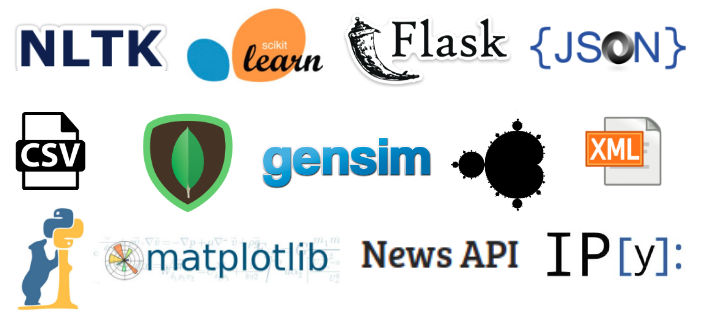
\includegraphics[height=150pt,width=320pt]{img/chapter4/tools/tools.png}
                    \caption{Logos de quelques librairies utilisées.}
                    \label{}
            \end{figure}
            \begin{enumerate}[leftmargin=*]
                \item{\textbf{NLTK : }}
                \textquotedbl Natural Language Toolkit\textquotedbl est une librairie Python destinée au TALN. Elle fournit une suite de bibliothèques de traitement de texte pour la classification, tokenization, stemming, étiquetage, analyse et raisonnement sémantique, etc. \cite{nltk}.\\

                \item{\textbf{Scikit-Learn : }}
                Bibliothèque libre et Open source implémentée avec Python, dédiée à l'apprentissage automatique. Elle est conçue pour s'harmoniser avec d'autres bibliothèques Python (ou autres), notamment NumPy, SciPy, etc. \cite{scikit}.\\

                \item{\textbf{Numpy : }}
                \textquotedbl Numerical Python\textquotedbl fournit une interface pour stocker et effectuer des opérations sur les données. D'une certaine manière, les tableaux Numpy sont comme les listes en Python, mais Numpy permet de rendre les opérations beaucoup plus efficaces, surtout sur les tableaux de grande taille qui sont au cœur de l'écosystème de la Data Science \cite{numpy}.\\

                \item{\textbf{Theano : }}
                bibliothèque Python qui permet de définir, d'optimiser et d'évaluer efficacement des expressions mathématiques impliquant des tableaux multidimensionnels. Ses principales caractéristiques sont la facilité d'intégration avec le module Numpy et l'utilisation transparente du GPU qui effectue des calculs intensifs plus rapidement qu'un CPU \cite{theano}.\\
                
                \item{\textbf{Gensim : }}
                Librairie Python gratuite conçue pour extraire automatiquement des sujets sémantiques à partir de documents. Les algorithmes de Gensim, tels que l'analyse sémantique latente, permettent de découvrir la structure sémantique des documents en examinant les schémas statistiques de cooccurrence des mots au sein d'un corpus de documents \cite{gensim}.\\

                \item{\textbf{Pandas : }}
                Fournis deux structures de données fondamentales, la \textquotedbl Série\textquotedbl et le \textquotedbl DataFrame\textquotedbl. On peut voir ces structures comme une généralisation des tableaux et des matrices de Numpy. La différence entre les structures de Pandas et celles de Numpy c'est la définition explicite par l'utilisateur des indices et des index sur les objets (matrices) \cite{pandas}.\\

                \item{\textbf{Pickle : }}
                Module Python utilisé pour sérialiser et désérialiser les structures d'objets Python. La sérialisation (ou «pickling») fait référence au processus de conversion d'un objet en mémoire en un flux d'octets pouvant être stocké sur disque ou envoyé sur un réseau. Plus tard, ce flux de caractères peut être récupéré et désérialisé (ou «unpickling») en retour vers un objet Python \cite{pickle}.\\

                \item{\textbf{Matplotlib : }}
                \textquotedbl Mathematic Plot library\textquotedbl est une bibliothèque de traçage Python 2D qui produit des figures de qualité de publication dans une variété de formats papier et d'environnements interactifs entre plates-formes. Matplotlib peut être utilisé dans les scripts Python, les Shells Python et IPython, les notebook Jupyter, etc. \cite{matplotlib}.\\

                \item{\textbf{Newspaper : }}
                Librairie Python accessible gratuitement qui permet d'extraire le contenu, l'image, les auteurs et la date de publication d'un article de presse en utilisant le protocole HTTP.\\

                \item{\textbf{Newsapi : }}
                Web API qui permet d'obtenir des articles de presse de dernière minute et de rechercher des articles de plus de 30 000 sources et blogs. Elle fournit également la possibilité de sélectionner les sources, les pays, les catégories, etc.\\

                \item{\textbf{FeedParser : }}
                \textquotedbl Universal Feed Parser\textquotedbl est une librairie Python pour le téléchargement et l'analyse des flux syndiqués connus sous l'appellation \emph{flux RSS}. Cette librairie se distingue par sa facilité d'utilisation \cite{feedparser}.\\

                \item{\textbf{TextBlob : }}
                Toolbox Python pour le traitement des données textuelles. Elle fournit une API simple permettant de plonger dans des tâches courantes de TALN, telles que l'étiquetage, l'extraction de syntagmes nominaux, l'analyse des sentiments, la classification, la traduction automatique, etc. \cite{textblob}.\\

                \item{\textbf{Farasa : }}
                L'équivalent arabe de \textquotedbl perspicacité\textquotedbl, Farasa est une Toolbox de traitement du langage naturel arabe développé au sein de l'institut \emph{Qatar Computing Research Institute}. Elle est composée de plusieurs modules : segmentation, étiquetage, etc. Farasa surpasse ou égalise les deux fameuses Toolbox pour l'arabe Stanford NLP et MADAMIRA \cite{farasa}.\\

                \item{\textbf{PyRouge : }}
                Interface Python pour le fameux module d'évaluation ROUGE des résumés automatiques. Elle facilite l'utilisation de ROUGE avec la conversion des fichiers qui contiennent les résumés en un format interprétable par ROUGE et génère automatiquement les fichiers de configuration ROUGE \cite{pyrouge}.\\

                \item{\textbf{PyMongo}}
                Module de gestion du SGBD MongoDB sous le langage Python, il fournit une variété de commandes très intéressantes qui permettent de faciliter la manipulation d'une base de données NoSQL \cite{pymongo}.\\

                \item{\textbf{Flask}}\label{flask}
                Framework open-source de développement web en Python. Son but principal est d'être léger, afin de garder la souplesse de la programmation Python, associé à un système de templates. Il est distribué sous licence BSD [Wikipédia].
            \end{enumerate}

        \subsubsection{Formats de données}
            \begin{enumerate}[leftmargin=*]
                \item{\textbf{XML : }}
                \textquotedbl eXtensible Markup Language\textquotedbl est un langage informatique de balisage générique. Ces balises permettent de structurer de manière hiérarchisée et organisée les données d'un document.\\

                \item{\textbf{JSON : }}
                \textquotedbl JavaScript Object Notation\textquotedbl est un format adapté aux types de données du langage JavaScript. Au cours des dernières années, JSON est devenu l'un des premiers formats d'échange et de stockage de données notamment pour le développement web \cite{jsonimpl}.\\
                
                \item{\textbf{CSV : }}
                \textquotedbl Comma-separated values\textquotedbl est un format informatique représentant des données tabulaires sous forme de valeurs séparées par des virgules. Le format de fichier CSV est utilisable par les applications de tableur KSpread, OpenOffice Calc, Microsoft Excel, etc. De nombreuses autres applications prennent en charge CSV pour importer ou exporter des données \cite{csv}.
            \end{enumerate}

        \subsubsection{Logiciels et éditeurs de textes}
            \begin{figure}[H]
                    \centering
                    
\includegraphics[height=80pt,width=250pt]{img/chapter4/tools/software.png}
                    \caption{Logos des logiciels utilisés.}
                    \label{}
            \end{figure}
            \begin{enumerate}[leftmargin=*]
                \item{\textbf{PyCharm Community Edition : }}
                PyCharm est un éditeur de code pour le développement sous Python. Il fournit la complétion de code intelligente, des inspections, la mise en évidence d'erreurs à la volée et des correctifs rapides, ainsi que des corrections de code automatisés et de riches fonctionnalités de navigation \cite{pycharm}. La version \emph{Community Edition} que nous avons utilisée est gratuite et en libre accès.\\

                \item{\textbf{WebStorm : }}
                WebStorm est un éditeur de code pour le développement sous Javascript. Il apporte une aide énorme aux développeurs web et mobile. Il supporte tous les langages compilés au JavaScript, Node.js, HTML et CSS \cite{webstorm}. Nous avons pu obtenir une licence étudiant d'une année.\\

                \item{\textbf{Sublime Text : }}
                Éditeur de texte générique codé en C++ et Python, il est disponible sur Linux, Mac et Windows. Depuis la version 2.0, sortie le 26 juin 2012, l'éditeur prend en charge 44 langages de programmation majeurs, tandis que des plugins sont souvent disponibles pour les langages plus rares \cite{sublime}. Nous avons utilisé la version d’essai qui est en libre accès sur internet.\\

                \item{\textbf{Git : }}
                Système de gestion de versions décentralisé. C'est un logiciel libre créé par \emph{Linus Torvalds}, auteur du noyau Linux, et distribué selon les termes de la licence publique générale (GPL). En 2016, il s’agit du logiciel de gestion de versions le plus populaire qui est utilisé par plus de douze millions de personnes \cite{git}.
            \end{enumerate}

\newpage
\section{Recommandation}

Afin d'implémenter cette approche et tenter de générer une collection de profils utilisateurs, nous avons essayé d'utiliser des datasets destinés aux articles de presse. Afin de concevoir une base de données de profils utilisateurs, nous avons sollicité \emph{Google News} \cite{bibid}, \emph{Bing News} \cite{bibid} et \emph{Yahoo Webscope} \cite{bibid} mais sans aucune réponse de la part de ces entreprises. Alors, nous avons exploré d'autres sources décrites ci-dessous.

\subsection{Corpus et dataset}
    \subsubsection{SmartMedia Adressa News Dataset}
    Le dataset Adressa est un ensemble de données d'actualité comprenant des articles de presse (en norvégien) associés à une base de profils utilisateurs. Cet ensemble de données est publié avec la collaboration de l'Université norvégienne des sciences et technologies \emph{(NTNU)} et \emph{Adressavisen} (journal local à Trondheim, Norvège) dans le cadre du projet \emph{RecTech} sur la technologie de recommandation \cite{refnorvege}.

    \begin{enumerate}[leftmargin=*]
        \item\textbf{Structure du dataset}\\
        Le dataset contient une collection d'articles et une collection d'utilisateurs. Les figures \ref{instance-profil} et \ref{instance-article} ci-dessous montrent la structure des collections de données.
        \begin{figure}[H]
            \centering
            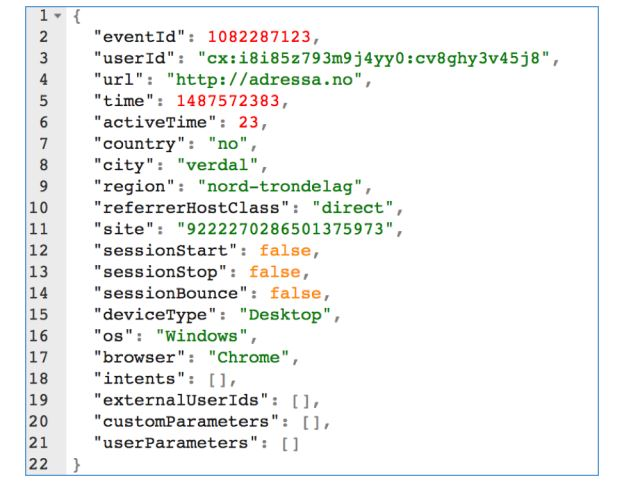
\includegraphics[width=350pt]{img/chapter4/smartmedia/structure_profil.jpg}
            \caption{Structure d'une instance de profil du dataset SmartMedia.}
            \label{instance-profil}
        \end{figure}
        
        \begin{figure}[H]
            \centering
            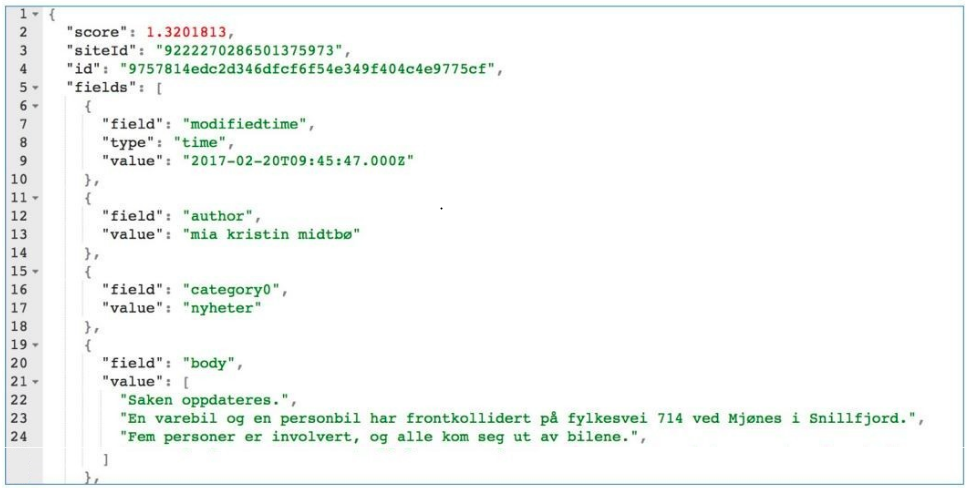
\includegraphics[width=410pt]{img/chapter4/smartmedia/structure.png}
            \caption{Structure d'une instance d'article du dataset SmartMedia.}
            \label{instance-article}
        \end{figure}

        \item\textbf{Statistiques sur le dataset}\\
        La récolte du dataset s'est faite pendant 7 jours pour une taille totale de 1.4 Go de collections d'articles et profils stockés dans des structures de format \emph{Json}. Il contient au total 923 articles et 15514 utilisateurs.\\

        \item\textbf{Inconvénients de l'utilisation de \textquotedbl SmartMedia Adressa News Dataset\textquotedbl}\\
        Le dataset décrit dans cette partie traite les articles de presse en langage norvégien, c'est à dire que les catégories des articles sont en norvégien et le contenu des articles aussi. Ceci nous a amenés à abandonner ce dataset. Ajouté à cela la masse importante de données que l'on ne peut modifier au risque de biaiser les résultats et la difficulté de traitements des fichiers dans un poste de travail (1 ou 2) ce qui nécessite l'utilisation du serveur.\\
    \end{enumerate}

    \subsubsection{\textquotedbl YOW \textquotedbl dataset }
    \emph{YOW} a été collecté à l'Université \emph{Carnegie Mellon} pour le \emph{Yow-now}, le système de filtrage des articles de presse \cite{carnegieYOW}. Le dataset YOW est composé de plusieurs attributs, des informations sur les interactions de 22 utilisateurs avec des articles de presse de différentes catégories. Les instances du dataset sont très bien adaptées au filtrage collaboratif. Comme il n'y a pas d'information sur le contenu des articles de presse, le filtrage basé sur le contenu n'est pas possible. \\
    \begin{enumerate}[leftmargin=*]
        \item\textbf{Structure du dataset}\\
        Chaque instance du dataset YOW est composée de 23 attributs propres à l'utilisateur et à l'article de presse. Ci-après les attributs les plus importants pour notre système de recommandations :  \\
\begin{lstlisting}[style=code] 
 {
 'user_id': '19', 
 'document_id': '27010084'
 'timestamp': '2004-04-23T15:38:25Z'
 'timeonpage': '63s', #temps de lecture
 'classes': [ 'space', 'international', 'iraq', ...],
 ...
 },
\end{lstlisting}
    \item\textbf{Statistiques sur le dataset}\\
    Yow-now est un système de filtrage d'informations qui recommande des articles de presse aux utilisateurs à partir de divers flux RSS. Les données sont recueillies par une étude d'un mois qui comprend environ 25 personnes et plus de 7000 entrées de commentaires de tous les utilisateurs. Au total 383 articles ont été évalués par chaque utilisateur. Le dataset comporte également des évaluations implicites et explicites sur les recommandations. Le profilage explicite est sous forme de note de 1 à 5; quant à l'implicite, il est établi selon les interactions de l'utilisateur (souris, clavier et activités de défilement).\\

    \item\textbf{Avantages de l'utilisation de \textquotedbl YOW Dataset\textquotedbl}\\
     Le dataset décrit dans cette partie traite les articles de presse en Anglais et contient des retours implicites de l'utilisateur. Ceci représente un avantage pour notre implémentation. De plus, le dataset est représenté dans un format \emph{CSV} qui est interprété rapidement par les postes de travail 1 et 2.\\
\end{enumerate}

    \subsection{Approche probabilité de sélection}  
    L'approche basée probabilité de sélection détaillée dans la \autoref{proba-selct} va être implémenté ci-dessous en utilisant le dataset \textquotedbl YOW\textquotedbl.
        \subsubsection{Recommandation personnalisée}
        \begin{enumerate}[leftmargin=*]
            \item\textbf{Pré-traitement des données}\\
            Chaque instance du dataset \emph{YOW} est une interaction de l'utilisateur U avec un article A. L'interaction peut avoir plusieurs valeurs pour l'attribut \emph{Classe} (catégorie dans notre cas). \textquotedbl Classe\textquotedbl peut prendre des noms de catégories et des mots-clés de l'article. Par exemple :
            \begin{itemize}
                \item Noms de catégories : world, science, entertainment, space, business, food, etc.
                \item Mots-clés : Iraq, Amazon, Malaysia, Oil, Japan, etc.\\ 
            \end{itemize}
            Pour adapter ces données à notre modèle de catégorisation d'article nous avons effectué des pré-traitements sur chaque instance du dataset. Nous avons annoté le dataset manuellement dans le but de convertir les noms de catégories et les mots-clés en catégories présentes dans notre système (7 pour l'Anglais et 6 pour l'Arabe). Par exemple :
            \begin{itemize}
                \item Avant : nuclear weapons, international, middle east, business, John Kerry, space, science.
                \item Après :
                \begin{itemize}
                    \item {nuclear weapons, international, middle east} : World
                    \item {John Kerry} : US
                    \item {space, science} : Science \& Technology
                    \item {accident, tradegy} : Society (Pour l'Anglais US)
                    \item {business} : Business\\
                \end{itemize}    
            \end{itemize}
            De plus, le dataset a été classé dans l'ordre croissant de l'attribut \textquotedbl Timestamp\textquotedbl, la date et l'horaire de l'interaction, dans le but de récupérer l'historique et le changement des centres d’intérêts de chaque utilisateur. 

            \item\textbf{Implémentation}\\
            À chaque nouvelle interaction, le vecteur de préférences de catégories d'un utilisateur se met à jour en fonction de la catégorie  de l'article visité. La mise à jour consiste en l'augmentation de la probabilité de sélection de la catégorie de l'article choisie et la diminution des autres catégories (s'il y en a). 
            L'exemple suivant montre le processus de mise à jour :
            \begin{itemize}[label={}]
                \item $P(U) = {'news': 0.0581,'sport': 0.717, 'sci\_tech': 0.149}$\\
            \end{itemize}

            L'utilisateur U a cliqué et lu un article de la catégorie \emph{Sport}, le vecteur de préférences de catégories va se mettre à jour en fonction de cette dernière interaction (détails dans \ref{proba-select}).
            \begin{itemize}[label={}]
                \item $P(U, sport) = (1-{\alpha}) * {P(U, sport)} + {\alpha}$
                \item $P(U, sport) = (1-{0.1}) * {P(U, sport)} + {0.1}$
                \item $P(U, sport) = (1-{0.1}) * {0.717} + {0.1}$
                \item $P(U, sport) = 0.745$
            \end{itemize}

            Quant aux autres catégories du vecteur de sélection :
            \begin{itemize}[label={}]
                \item $P(U, news) = (1-{\alpha}) * {P(U, news)} $
                \item $P(U, news) = (1-{0.1}) * {P(U, news)} $
                \item $P(U, news) = (1-{0.1}) * {0.0581} $
                \item $P(U, news) = 0.0523$
                \item 
                \item $P(U, sci\_tech) = (1-{\alpha}) * {P(U, sci\_tech)} $
                \item $P(U, sci\_tech) = (1-{0.1}) * {P(U, sci\_tech)} $
                \item $P(U, sci\_tech) = (1-{0.1}) * {0.1499} $
                \item $P(U, sci\_tech) = 0.135$
            \end{itemize}
            Après cette interaction, le vecteur de préférences de catégories de l'utilisateur U devient :
            \begin{itemize}[label={}]
                \item $P(U) = {'news': 0.0523, 'sport': 0.745, 'sci_tech': 0.135}$\\
            \end{itemize}
            Pour un nouvel utilisateur, le même traitement est appliqué. Ainsi le vecteur de préférences de catégories se remplit petit à petit en fonction des interactions qui vont être mises à jour de la même façon. Cela résout le problème de démarrage à froid (\autoref{cold-start}).
        \end{enumerate}

        \subsubsection{Recommandation non personnalisée}
        Dans le cas où l'utilisateur n'est pas connecté, il ne possède pas de vecteur de préférences de catégories, et donc la recommandation sera basée sur la similarité entre articles.
            \begin{enumerate}[leftmargin=*]
                \item\textbf{Implémentation}\\
                Si l'utilisateur U a lu l'article A\textsubscript{1}, les articles A\textsubscript{2}, A\textsubscript{3}, ..., A\textsubscript{n} similaires à A\textsubscript{1}, seront recommandés. La similarité entre articles est calculée à partir du contenu. Le texte sera converti en TF-IDF et les articles les plus proches, en calculant la similarité de Cosinus, seront considérés comme articles qui parlent du même sujet ou de la même catégorie.

                 Exemple : A\textsubscript{1} = \textquotedbl Real Madrid 3-1 Liverpool: Jurgen Klopp says Reds wanted everything and got minus something\textquotedbl\\
                    Articles similaires à A\textsubscript{1} = \{
                    \textquotedbl Gareth Bale on his Champions League final goal for Real Madrid\textquotedbl: 0.26435,\\
                    \textquotedbl Real Madrid 3-1 Liverpool: Flawed Karius pays for lack of focus \textquotedbl: 0.21839,\\
                    \textquotedbl Columbus Crew: Two US cities fight over one football team\textquotedbl: 0.073586
                    \}
                \end{enumerate}
    \subsection{Intégration du module de recommandation}
   Dans la phase d'intégration, nous avons implémenté les algorithmes de recommandation et utilisé les bases de profil dans notre serveur en utilisant la bibliothèque PyMongo. Ainsi, dans chacun des processus de recommandation, les mises à jour seront faites automatiquement au niveau de notre base de données stockée sur le serveur.

\section{Catégorisation d'articles}
Le deuxième module sur lequel nous avons travaillé, est la catégorisation d'articles de presse. Nous avons expérimenté plusieurs techniques proposées dans la littérature. Nous présentons ci-après chaque approche, ses résultats, ses points forts et ses faiblesses.

Toutes les approches utilisées sont basées sur l'apprentissage automatique, supervisé et non supervisé. 
    \subsection{Approche basée sur l'apprentissage non supervisé LDA}
    Nous avons utilisé la technique \textquotedbl Latent Dirichlet Allocation\textquotedbl, déjà présentée dans la \autoref{non-supervised}.

    \begin{enumerate}
        \item \textbf{Corpus et dataset :}\\
        Comme expliqué dans le chapitre précédent (\autoref{non-supervised}), nous avons utilisé le dataset CNN qui contient 92000 articles pour implémenter et évaluer le modèle d'apprentissage non supervisé.

        \item \textbf{Implémentation :}\\
        Pour l'implémentation de \emph{LDA} nous avons utilisé la bibliothèque Gensim pour : la racinalisation, le stemming, l'extraction des caractéristiques, et l'implémentation du modèle. 

        \item \textbf{Évaluation du modèle :}\\
        Après avoir entrainé notre modèle sur plusieurs paramètres, nous avons retenu les meilleurs :\\
        Nombre de passes : 10, Nombre de topics : 14, Nombre d'itérations par passe : 1000. 
    \end{enumerate}

    Nous avons obtenu ci-dessous une représentation, selon le nombre de sujets définis, une liste des mots les plus représentatifs (10 mots) de chaque cluster pour un échantillon de 6 clusters.
    \begin{table}[H]
        \begin{center}
            \begin{tabular}{|C{2.1cm}|C{2.1cm}|C{2.1cm}|C{2.1cm}|C{2.1cm}|C{2.1cm}|}
                \hline                      
                \textbf{Health} & \textbf{Tech.} & \textbf{World} & \textbf{Travel} & \textbf{US} & \textbf{Justice}\\ 
                \hline     
                health &  facebook &         china  &    world  &     president   &   court \\
                school  &     news  &   government  &     city     &      obama  &     case \\
                children  &    media   &       north  &   london     &       u.s.  & attorney \\  
                students  &   online   &      united  &     park     &     states  &  charges \\  
                medical  &    video   &        u.s.  &    south     &   american  &    judge \\  
                care  &  twitter   &        iran  &    hotel     &      white  &      law \\  
                university  &   social   &      australia  &  british     &     united  & trial \\ 
                hospital &  internet   &      russia   &    year   &   government  &   report \\  
                disease   &     use   &       korea   &     art & house  &    told  \\  
                parents   &   phone & continent &   africa    &     america  &   prison \\  
                \hline
                
            \end{tabular}
        \end{center}
        \caption{Résultats des clusters résultant de la catégorisation en Anglais avec LDA.}
        \label{Lda-categ}
    \end{table}                           

    Après avoir explicité la liste des mots par cluster, ci-dessous, nous allons présenter les résultats de l'évaluation du modèle \emph{LDA} présenté dans \ref{inmplementation}.
    \begin{table}[H]
        \begin{center}
            \begin{tabular}{|c|c|}
                \hline
                \textbf{Perplexité} & \textbf{Cohérence de sujet} \\
                \hline
                -8.560 &-1.572  \\
                \hline
            \end{tabular}
        \end{center}
        \caption{Évaluation du modèle LDA}
        \label{Eval LDA}
    \end{table}

    Le tableau ci-dessus présente les résultats obtenu (perplexité et cohérence de sujet) par l'algorithme LDA.

    Néanmoins, l'inconvénient majeur de LDA est le temps de prédiction. Pour prédire la catégorie d'un article, LDA doit charger le dictionnaire contenant tout le vocabulaire plus le vocabulaire de l'article à prédire. Après cela, le modèle lui-même est mis à jour pour permettre de prédire la catégorie. Ce qui n'est pas très optimal pour une utilisation dans une application qui doit gérer plusieurs modèles à la fois.


\subsection{Approches basées sur l'apprentissage supervisé}
La catégorisation d'articles de presse basée sur l'apprentissage supervisé nécessite un corpus d'articles déjà annotés avec les catégories de chaque document. Nous présentons ci-après les étapes suivies dans le développement du modèle de catégorisation par apprentissage supervisé d'articles de presse.

\subsection{Corpus et dataset}
Comme tout problème de classification, la catégorisation d'articles de presse nécessite de très grandes masses de données. C'est pour cela que nous avons  consacré une bonne période du projet à la récolte des corpus et la préparation des datasets.     

    \subsubsection{Anglais}
    Le dataset baptisé \textquotedbl News\textquotedbl a été récolté par le Laboratoire Informatique de \emph{l'Université de Pise} \cite{pise}. Il regroupe des articles de 3 sources différentes : \emph{The New York Times}, \emph{Reuters} et \emph{USA Today}. le Tableau \ref{news-categ} présente en détail le nombre d'articles de chaque catégorie.
    \begin{table}[H]
        \begin{center}
            \begin{tabular}{|C{5cm}|C{5cm}|}
                \hline
                \textbf{Catégorie} &  \textbf{Nombre d'articles} \\
                \hline
                Business & 5366 \\                            
                Entertainment & 3286 \\
                Health & 1851 \\
                Science \& Technology & 2872 \\
                Sport & 8189 \\
                US & 4783 \\
                World & 6255 \\
                \textbf{Totale} &  \textbf{32602} \\
                \hline
            \end{tabular}
        \end{center}
        \caption{Nombres d'articles de chaque catégorie du corpus \textquotedbl News\textquotedbl}
        \label{news-categ}
    \end{table}

    \subsubsection{Arabe}
    Le corpus TALAA\footnote{Développé par l'équipe de recherche Traitement Automatique du Langage et Apprentissage Automatique du Laboratoire de Recherche en Intelligence Artificielle du département informatique de l'USTHB} pour la catégorisation d'articles de presse est une grande collection d'articles publiés entre 2010 et 2014 dans différentes revues de presse arabes sur internet. Il contient plus de 14 millions de mots de 582000 types différents. Le corpus contient 8 catégories, mais nous avons choisi de travailler sur 6 catégories plus générales comme on peut le constater dans le \autoref{talaa-categ} \cite{asma-sellab}. 
    \begin{table}[H]
        \begin{center}
            \begin{tabular}{|c|c|}
                \hline
                \textbf{Catégorie} &  \textbf{Nombre d'articles} \\
                \hline
                \begin{arab}الجزائر\end{arab} & 6603 \\
                \begin{arab}الثقافة\end{arab} & 3311 \\
                \begin{arab}الدين\end{arab} & 2568 \\
                \begin{arab}المجتمع\end{arab} & 7714 \\
                \begin{arab}الرياضة\end{arab} & 8104 \\
                \begin{arab}العالم\end{arab} & 4380 \\
                \textbf{Totale} & \textbf{32680} \\
                \hline
            \end{tabular}
        \end{center}
        \caption{Nombres d'articles des 6 catégories choisies du corpus \textquotedbl TALAA\textquotedbl}
        \label{talaa-categ}
    \end{table}

\subsection{Pré-traitement et structure des datasets}
Les deux corpus utilisés dans les deux langues étaient sous format brut, ce qui nécessitait une restructuration et un pré-traitement afin de permettre leur exploitation. Plusieurs opérations de pré-traitements ont été effectuées. Ci-après les étapes suivies :

\begin{enumerate}
    \item{\textbf{Segmentation (Tokenization) et suppression des mots vides :} } Pour l'Anglais nous avons utilisé le Tokenizer natif de NLTK, et la FARASA Toolbox pour la langue Arabe.\\  
    
    \item{\textbf{Racinisation (Stemming) :} } 
    La librairie Snowball Stemmer de NLTK a été utilisée pour l'Anglais; quant à l'Arabe c'est toujours la Toolbox FARASA.\\
    
    \item{\textbf{N-grammes :} }
    L'algorithme natif de NLTK a été utilisé pour les deux langues (Anglais et Arabe).\\ 
    
    \item{\textbf{Extraction des caractéristiques :} }
    Les librairies Countvectorizer et tfidfvectorizer de scikit-learn ont été utilisés dans l'extraction des caractéristiques pour l'Anglais et l'Arabe.\\
\end{enumerate}


\subsection{Implémentation}
Après expérimentation des techniques citées dans la \autoref{approches}, voici les modèles finaux de la catégorisation d'articles de presse implémentés en Python en utilisant la librairie Scikit-learn (\autoref{def-tools}) :

    \subsubsection{Corpus Anglais}
    le modèle le plus performant est obtenu en utilisant l'algorithme SVM avec 80\% de données pour l'apprentissage et les 20\% restants pour les tests sur un total de 32602 articles de 7 catégories différentes.
    
    Le \autoref{modele-categ-en}, présente une comparaison entre les deux techniques expérimentées pour l'Anglais.
    \begin{table}[H]
        \begin{center}
            \begin{tabular}{|l|C{6cm}|r|} 
                \hline
                \textbf{Modèle} & \multicolumn{2}{c|}{\textbf{Résultats}} \\
                \hline
                    & Précision & \textbf{0.99} \\
                \textbf{SVM} & Rappel & \textbf{0.99} \\
                    & F-mesure & \textbf{0.99} \\
                \hline
                LDA & Perplexité & -8.55 \\
                    & Cohérence & -1.57 \\
                \hline
            \end{tabular}
        \end{center}
        \caption{Résultats comparatifs des modèles de catégorisation pour l'arabe}
        \label{modele-categ-en}
    \end{table}
      
    \subsubsection{Corpus Arabe}
    l'algorithme de la Descente de Gradient Stochastique nous a donné les meilleurs résultats en utilisant 32680 articles, avec 75\% de données pour l'apprentissage et le reste pour les tests. 

    Le \autoref{modele-categ-ar} présente une comparaison entre les résultats des différentes techniques expérimentées.
    \begin{table}[H]
      \begin{center}
          \begin{tabular}{|c|c|c|c|c}
              \hline
              \textbf{Modèle} & \textbf{Précision} & \textbf{Rappel} & \textbf{F-mesure} \\
              \hline
              Naïve de Bayes & 0.89 & 0.87 & 0.88 \\
              Arbre de décision & 0.82 & 0.84 & 0.83 \\
              \textbf{Descente de Gradient Stochastique} & \textbf{0.94} & \textbf{0.94} & \textbf{0.94} \\
              SVM & 0.91 & 0.89 & 0.90 \\
              \hline
          \end{tabular}
      \end{center}
      \caption{Résultats comparatifs des modèles de catégorisation pour l'arabe}
      \label{modele-categ-ar}
    \end{table}  

\subsection{Résultats}\label{result-categ}
    Les résultats des tests des modèles de catégorisation d'articles de presse sont calculés en utilisant les métriques déjà présentées dans la \autoref{metrics}. Des résultats comparatifs sont présentés dans ce qui suit.
    \subsubsection{Anglais}
    Le modèle destiné à la catégorisation d'articles de presse de l'Anglais a montré une très haute capacité prédictive, l'exactitude du meilleur modèle est de 98,7\%. Le \autoref{result-categ-en} présente les résultats détaillés de chaque catégorie avec les mesures de performances.
    % \begin{itemize}
    %   \item{Accuracy : 0.987}
    %   \item{Précision : 0.988}
    %   \item{Rappel : 0.982}
    %   \item{F-mesure : 0.985}
    % \end{itemize}
    \begin{table}[H]
        \begin{center}
            \begin{tabular}{|c|C{2cm}|C{2cm}|C{2cm}|C{2cm}|}
                \hline
                \textbf{Catégorie} &  \textbf{Précision} &  \textbf{Rappel} &  \textbf{F-mesure} &  \textbf{Support} \\
                \hline
                Business & 0.98 & 0.96 & 0.97 & 1046 \\
                Entertainment & 0.99 & 0.99 & 0.99 & 651 \\
                Health & 0.97 & 1.00 & 0.99 & 388 \\
                Science \& Technology & 0.94 & 1.00 & 0.97 & 546 \\
                Sport & 1.00 & 1.00 & 1.00 & 1635 \\
                US & 0.99 & 0.98 & 0.99 & 993 \\
                World & 1.00 & 0.99 & 0.99 & 1262 \\                          
                \textbf{Final} & \textbf{0.99} & \textbf{0.98} & \textbf{0.99} & \textbf{6521} \\
                \hline
            \end{tabular}
        \end{center}
        \caption{Résultat global et pour chaque catégorie de la catégorisation pour l'Anglais.}
        \label{result-categ-en}
    \end{table}

    \subsubsection{Arabe}
    Le modèle de catégorisation d'articles de presse arabe a montré, également, des résultats très satisfaisants avec une accuracy de 93.6\% et une précision de 94\%. Les résultats détaillés sont présentés dans le \autoref{result-categ-ar}.
    % \begin{itemize}
    %   \item{Accuracy : 0.936}
    %   \item{Précision : 0.94}
    %   \item{Rappel : 0.94}
    %   \item{F-mesure : 0.94}
    % \end{itemize}
    \begin{table}[H]
        \begin{center}
            \begin{tabular}{|c|C{2cm}|C{2cm}|C{2cm}|C{2cm}|}
                \hline
                \textbf{Catégorie} &  \textbf{Précision} &  \textbf{Rappel} &  \textbf{F-mesure} &  \textbf{Support} \\
                \hline
                \begin{arab}الجزائر\end{arab} & 0.93 & 0.88 & 0.91 & 664 \\
                \begin{arab}الثقافة\end{arab} & 0.91 & 0.86 & 0.88 & 509 \\
                \begin{arab}الدين\end{arab} & 0.94 & 0.92 & 0.93 & 860 \\
                \begin{arab}المجتمع\end{arab} & 0.91 & 0.94 & 0.92 & 1541 \\
                \begin{arab}الرياضة\end{arab} & 0.99 & 0.99 & 0.99 & 1620 \\
                \begin{arab}العالم\end{arab} & 0.92 & 0.94 & 0.93 & 1316 \\                      
                \textbf{Final} & \textbf{0.94} & \textbf{0.94} & \textbf{0.94} & \textbf{6510} \\
                \hline
            \end{tabular}
        \end{center}
        \caption{Résultat global et pour chaque catégorie de la catégorisation pour la langue Arabe}
        \label{result-categ-ar}
    \end{table}

\subsection{Évaluations}
    \subsubsection{Anglais}
    Le \autoref{confusion-anglais} présente la matrice de confusion du module de catégorisation d'articles de presse pour l'Anglais. On peut constater qu'il y a très peu de confusion entre les différentes catégories, à part quelques articles comme les 31 articles qui ont été prédits comme \emph{Science \& Technology} alors qu'ils appartiennent à la catégorie \emph{Business}. Cela est dû au contenu de ces articles qui parlent de business dans le domaine de la science et technologie. 
    \begin{table}[H]
        \begin{center}
            \begin{tabular}{|c|c|c|c|c|c|c|c|}
                \cline{2-8}
                \multicolumn{1}{c|}{} & \textbf{Sport} &  \textbf{World} &  \textbf{News} &  \textbf{Business} &  \textbf{Health} & \textbf{Entert.\footnote{Entertainment}} &  \textbf{Sci-Tech} \\
                \hline
                \textbf{Sport} & 1635 & 0 & 0 & 0 & 0 & 0 & 0 \\
                \textbf{World}  & 0 & 1249 & 0 & 9 & 2 & 1 & 1 \\
                \textbf{News}  & 0 & 0 & 974 & 11 & 3 & 3 & 2 \\
                \textbf{Business}  & 0 & 5 & 4 & 1003 & 3 & 0 & 31 \\
                \textbf{Health}  & 0 & 0 & 0 & 0 & 388 & 0 & 0 \\
                \textbf{Entert.}  & 0 & 0 & 0 & 1 & 3 & 646 & 1 \\
                \textbf{Sci-Tech}  & 0 & 0 & 1 & 0 & 0 & 1 & 544 \\
                \hline
            \end{tabular}
        \end{center}
        \caption{Matrice de confusion du modèle de catégorisation d'articles de presse pour la langue Anglaise}
        \label{confusion-anglais}
    \end{table}
   Les données de la matrice de confusion sont représentées graphiquement dans la \autoref{roc-en} sous forme de courbe ROC (Receiver Operating Characteristic) qui donne le taux de vrais positifs en fonction du taux de faux positifs.
    \begin{figure}[H]
        \centering
        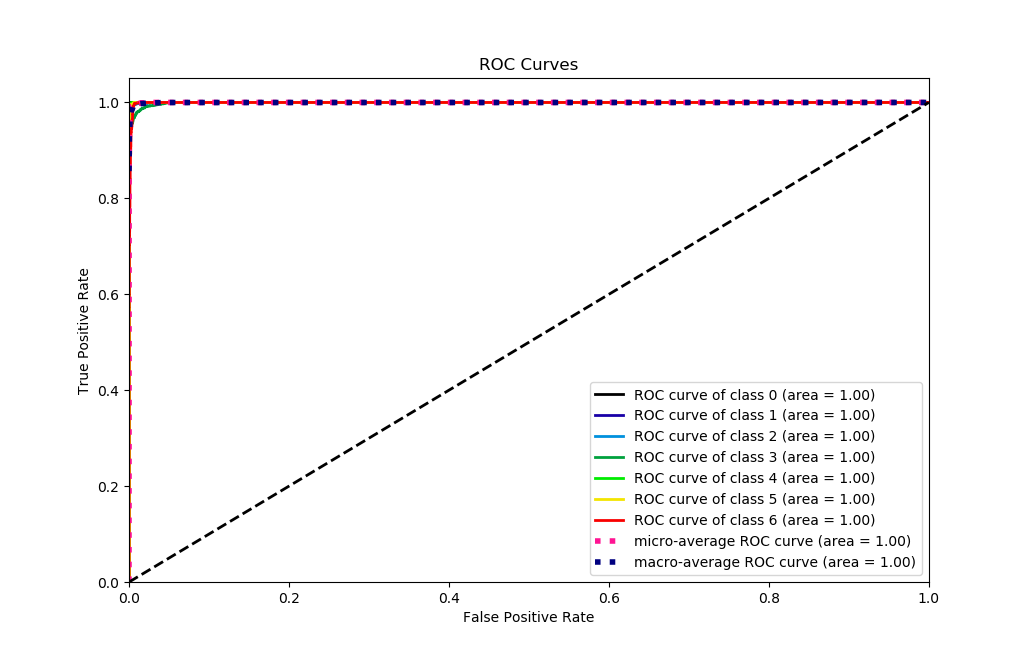
\includegraphics[height=320pt,width=330pt]{img/chapter4/result/rocEN.png}
        \caption{Courbe ROC du modèle de catégorisation d'articles de presse pour la langue Anglaise}
        \label{roc-en}
    \end{figure}

    \subsubsection{Arabe}
    Tout comme pour l'Anglais, le modèle développé pour l'Arabe a montré une capacité de prédiction très élevée. Comme on peut le voire dans le \autoref{confusion-arabe}, la confusion entre les catégories est très faible à part quelques articles des catégories proches en terme de contenu. 
    \begin{table}[H]
        \begin{center}
            \begin{tabular}{|c|c|c|c|c|c|c|}
                % \cline{2-7}
                % \hline
                % \multicolumn{1}{c|}{} & \multicolumn{6}{|c|}{Predicted} \\
                % \hline
                \cline{2-7}
                \multicolumn{1}{c|}{} & \textbf{\begin{arab}العالم\end{arab}} &  \textbf{\begin{arab}الرياضة\end{arab}} &  \textbf{\begin{arab}الجزائر\end{arab}} &  \textbf{\begin{arab}المجتمع\end{arab}} &  \textbf{\begin{arab}الدين\end{arab}} &  \textbf{\begin{arab}الثقافة\end{arab}} \\
                \hline
                \textbf{\begin{arab}العالم\end{arab}} & 1232  &  1  & 11 &  51  & 18  &  3 \\
                \textbf{\begin{arab}الرياضة\end{arab}}  & 1 & 1609  &  1  &  6  &  3 &   0 \\
                \textbf{\begin{arab}الجزائر\end{arab}}  & 28  &  2 & 587 &  21  &  9  & 17 \\
                \textbf{\begin{arab}المجتمع\end{arab}}  & 43  & 11 &  17& 1447 &  12 &  11 \\
                \textbf{\begin{arab}الدين\end{arab}}  & 36  &  0  &  6 &  18 & 788 &  12 \\
                \textbf{\begin{arab}الثقافة\end{arab}}  & 3  &  0 &   8 & 53  &  9 & 436 \\
                \hline
            \end{tabular}
        \end{center}
        \caption{Matrice de confusion du modèle de la catégorisation d'articles Arabe.}
        \label{confusion-arabe}
    \end{table}

    La courbe ROC du modèle de catégorisation pour la langue arabe est présentée dans la \autoref{roc-ar} 
    \begin{figure}[H]
        \centering
        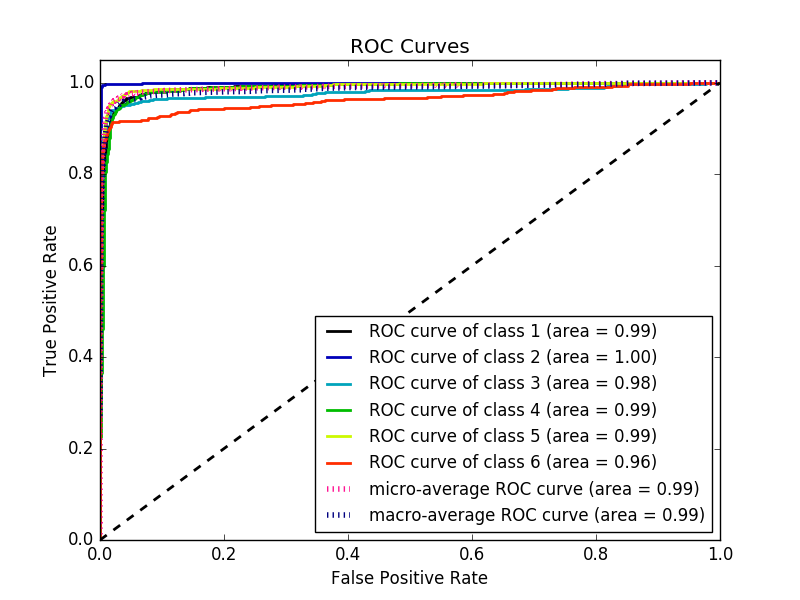
\includegraphics[height=320pt,width=330pt]{img/chapter4/result/rocAR.png}
        \caption{Courbe ROC du modèle de catégorisation pour la langue arabe.}
        \label{roc-ar}
    \end{figure}

    Après toutes les expérimentations, nous avons conclu que les modèles basés sur l'apprentissage supervisé sont plus performants et ont données de très bon résultats. Les résultats sont présentés dans la \autoref{result-categ}.
    
\subsection{Intégration du module de catégorisation}
Afin d'intégrer notre module de catégorisation, nous avons utilisé la bibliothèque Pickle qui permet de sauvegarder le modèle dans un fichier binaire. Ensuite, il suffit juste de charger le modèle et de lancer la prédiction sur de nouveaux articles.


\section{Résumé automatique}
La deuxième partie de la phase de réalisation est consacrée au résumé automatique. Nous avons expérimenté plusieurs techniques et méthodes que nous allons voir en détail dans cette section. 
\subsection{Résumé extractif par Apprentissage Supervisé}
Nous avons commencé par une approche basée sur l'apprentissage automatique supervisé, ce qui nécessitait des corpus d'articles avec leurs résumés types.

    \subsubsection{Contribution à la récolte de données : \textquotedbl Sumrized\textquotedbl et \textquotedbl Mou3in\textquotedbl}
    Face au manque flagrant des corpus (gratuits) pour le résumé automatique, nous avons développé une plate-forme contributive sur le web baptisée \textbf{Sumrized.com} pour la récolte des textes et des résumés en trois langues l'Arabe, l'Anglais et le Français.
    
    Chaque texte et son résumé sont vérifiés manuellement par un expert qui peut consulter et valider les contributions à partir d'un Dashboard dédié à cet effet. L'interface principale de la plate-forme, qui est en ligne depuis février 2018, est présentée dans la figure \ref{sumrized-ui}. 
    
    \begin{figure}[H]
        \centering
        
\includegraphics[height=180pt,width=320pt]{img/chapter4/sumrized/responsive.png}
        \caption{La plate-forme Sumrized sur les différents supports}
        \label{sumrized-ui}
    \end{figure} 
    
    Nous avons également développé une application de bureau, appelée \textbf{Mou3in}, afin de faciliter l'annotation des textes. Elle offre à son utilisateur la possibilité d'attribuer une étiquette à chaque phrase selon son jugement (à supprimer ou à laisser). La figure \ref{mou3in} présente l'espace de travail sur l'application \textquotedbl Mou3in\textquotedbl :
    \begin{figure}[H]
        \centering
        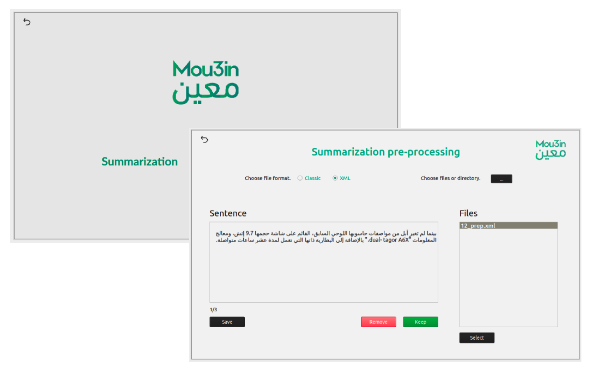
\includegraphics[height=230pt,width=370pt]{img/chapter4/mou3in/mou3in.png}
        \caption{Interface utilisateur de \textquotedbl Mou3in\textquotedbl}
        \label{mou3in}
    \end{figure}
    
    L'approche basée sur l'apprentissage automatique demandait un très grand nombre d'articles résumés, ce qui nous a poussés à l'abandonner.


\subsection{Résumé extractif par Machine de Boltzman}
L'approche proposée dans \cite{boltzman} utilise un modèle d'apprentissage profond afin de prédire les phrases les plus importantes dans un texte donné en utilisant 9 caractéristiques sur chaque phrase. Elle consiste en trois grandes phases: l'extraction des caractéristiques, la conversion en valeurs numériques et la génération du résumé à partir des scores de chaque phrase. 

    \subsubsection{Pré-traitement et structure du dataset}
    Cette méthode, contrairement aux autres, est appliquée sur un seul document et n'a pas besoin de plusieurs documents. La texte est segmenté en phrases, chaque phrase est divisée en mots, et les caractéristiques citées ci-dessus sont calculées.\\
    
    La matrice qui représente le texte est injectée dans une Machine de Boltzman\footnote{Type de réseau de neurones artificiels pour l'apprentissage non supervisé} en utilisant la bibliothèque Theano \cite{theano} afin de calculer les scores des phrases. Les résultats sont triés dans l'ordre décroissant des scores et le résumé est établi selon ces derniers.\\
    
    \subsubsection{Résultats et critiques}
    L'évaluation de ce modèle a été effectuée en utilisant le \emph{Gold Standard}\footnote{Dataset de référence construit par des experts linguistes, utilisé pour l'évaluation des résultats} Duc2004 qui est un dataset qui contient 50 articles de presse de différentes catégories et 4 à 5 résumés de référence pour chaque article.
    
    Afin d'évaluer notre résumeur automatique, nous avons appliqué le paramètre suivant :
    
    Longueur du résumé = 25 \% de la taille du texte en entrée.
    
    Nous avons obtenu les résultats présentés dans le \autoref{result-boltzman} en utilisant ROUGE (définie dans le chapitre précédent dans la \autoref{metrique-eval}) : 
    \begin{table}[H]
        \begin{center}
            \begin{tabular}{|c|C{1.2cm}|C{1.2cm}|C{1.2cm}|C{1.2cm}|C{1.2cm}|C{1.2cm}|C{1.2cm}|C{1.2cm}|}
                \cline{2-9}
                \multicolumn{1}{c|}{} & \textbf{R-1} &  \textbf{R-2} &  \textbf{R-3} &  \textbf{R-4} &  \textbf{R-L} &  \textbf{R-W} &  \textbf{R-S} &  \textbf{R-SU} \\
                \hline
                \textbf{Rappel} & 0.4172 & 0.0615 & 0.0129 & 0.0042 & 0.3239 & 0.1089 & 0.1693 & 0.1739 \\
                \textbf{Précision} & 0.1982 & 0.0264 & 0.0054 & 0.0016 & 0.1525 & 0.0919 & 0.0385 & 0.0402 \\
                \textbf{F-mesure} & 0.2549 & 0.0346 & 0.0071 & 0.0022 & 0.1963 & 0.0934 & 0.0556 & 0.0578 \\
                \hline
            \end{tabular}
        \end{center}
        \caption{Résultats du résumeur extractif basé sur la Machine de Boltzman}
        \label{result-boltzman}
    \end{table}
    En effet, ces résultats sont très proches des résumeurs de l'état de l'art, mais le modèle que nous avons utilisé est pré-entraîné sur un type de données totalement différent (des images), ce qui nous a amenés à laisser tomber cette approche.   

\subsection{Résumé extractif par Plongement de mots}
Dans ce type de résumé, nous allons appliquer le modèle de plongements de mots pré-entraîné de Wikipédia \cite{fasttext} sur un document (Résumeur automatique extractif mono document) \cite{notreresume} afin d'aboutir à un résumé automatique et cela en utilisant les bibliothèques Gensim et NumPy. 

\subsection{Résultats et évaluation}
Afin d'évaluer ce résumeur automatique, nous avons utilisé le dataset Duc2004 et nous avons fixé les paramètres suivants :

Seuil de similarité = 0.95, Seuil de poids du document (IDF) = 0.3, et la longueur du résumé = 25 \% de la taille du texte en entrée.

Nous avons obtenu les résultats présentés dans le \autoref{result-boltzman} en utilisant ROUGE. 

\begin{table}[H]
    \begin{center}
        \begin{tabular}{|c|C{1.2cm}|C{1.2cm}|C{1.2cm}|C{1.2cm}|C{1.2cm}|C{1.2cm}|C{1.2cm}|C{1.2cm}|}
            \cline{2-9}
            \multicolumn{1}{c|}{} & \textbf{R-1} &  \textbf{R-2} &  \textbf{R-3} &  \textbf{R-4} &  \textbf{R-L} &  \textbf{R-W} &  \textbf{R-S} &  \textbf{R-SU} \\
            \hline
            \textbf{Rappel} & 0.5631 & 0.1226 & 0.0346 & 0.0139 & 0.5111 & 0.1729 & 0.2981 & 0.3029 \\
            \textbf{Précision} & 0.1662 & 0.0361 & 0.0105 & 0.0042 & 0.1503 & 0.0912 & 0.0281 & 0.0289 \\
            \textbf{F-mesure} & 0.2485 & 0.0541 & 0.0157 & 0.0063 & 0.2245 & 0.1145 & 0.0488 & 0.0503 \\
            \hline
        \end{tabular}
    \end{center}
    \caption{Résultats du résumeur extractif basé sur le plongement de mots}
    \label{result-boltzman}
\end{table}

L'évaluation de résumeur montre une augmentation des valeurs des métriques d'évaluation par rapport à l'approche précédente qui est moins performante sur le même dataset. Ces résultats nous en poussé à considérer le résumeur automatique basé sur les plongements de mots comme résumeur du système \textquotedbl Feedny\textquotedbl.

\subsection{Intégration du module de résumé autmatique}
Dans la phase d'intégration, nous avons charger les modèles de plongement de mots (Anglais et Arabe) comme modèles de résumé automatique et nous avons fait appel dans notre serveur.

\section{Traduction automatique}
Comme il a été décrit dans le chapitre précédent, la traduction automatique sera intégrée directement à l'application finale afin d'offrir une fonctionnalité de traduction en plus de celle du résumé et de la catégorisation. À cet effet, nous avons utilisé la bibliothèque TextBlob \autoref{def-tools} qui offre une traduction multilingue d'un article ou d'un résumé.

\subsection{Traduction automatique par TextBlob}
\begin{itemize}
    \item Anglais :\\ 
    \textquotedbl The Interior Ministers of Spain and Algeria signed an agreement this week to form a joint team of investigation with the goals of fighting \textquotedbl illegal migration\textquotedbl and \textquotedbl preventing terrorism\textquotedbl. The agreement comes after recent crackdowns by the Algerian authorities during the first months of 2018 have reduced the number of undocumented Algerian migrants arriving in Spain, a reduction that was praised by the Spanish Interior Minister Juan Ignacio Zoido at their meeting in Madrid.\textquotedbl \\
    
    \item Arabe :\\
    \begin{arab}" وقع وزيرا الداخلية الإسباني والجزائري اتفاقا هذا الأسبوع لتشكيل فريق مشترك من التحقيق بهدف محاربة "الهجرة غير الشرعية" و "منع الإرهاب". ويأتي هذا الاتفاق بعد الإجراءات القمعية الأخيرة التي قامت بها السلطات الجزائرية خلال الأشهر الأولى من خفّض عام 2018 عدد المهاجرين الجزائريين غير الشرعيين الذين وصلوا إلى إسبانيا ، وهو تخفيض أشاد به وزير الداخلية الإسباني خوان إغناسيو زويدو في اجتماعهم في مدريد. "\end{arab}
    
    \item Français :\\
    \textquotedbl Les ministres de l'Intérieur d'Espagne et d'Algérie ont signé cette semaine un accord pour former une équipe conjointe d'enquête ayant pour objectif de lutter contre les \textquotedbl migrations clandestines\textquotedbl et \textquotedbl la prévention du terrorisme\textquotedbl. L'accord intervient après les récentes mesures de répression des autorités algériennes. 2018 ont réduit le nombre de migrants algériens sans papiers arrivant en Espagne, une réduction qui a été saluée par le ministre espagnol de l'Intérieur Juan Ignacio Zoido lors de leur réunion à Madrid.\textquotedbl \\
\end{itemize}

Comme mentionné dans le chapitre précédent, les traductions obtenues ont été jugées très bonnes, suffisamment pour pouvoir utiliser le traducteur TextBlob.

\subsection{Intégration du module de traduction automatique}
L'intégration du module de traduction se fait juste sur un appel depuis l'API du système \textquotedbl Feedny\textquotedbl en utilisant la bibliothèque TextBlob et en fournissant les langages source et cible en paramètres.


\section{Présentation de l'application \textquotedbl Feedny\textquotedbl}
Après avoir finalisé les différents modules qui composent notre système, nous avons procédé à l'intégration de ces derniers dans une application mobile multiplate-forme (Androïd et IOS) dans l'optique de permettre à l'utilisateur de bénéficier de chaque fonctionnalité.!!

% L'expérience utilisateur au sein de notre application est étudier pour optimiser la navigation entre les différents espaces. L'application est très intuitifs et conçu afin d'attirer les utilisateurs le plus de temps possible.
La phase d'implémentation a été divisée en deux parties, le développement Back-end de l'API qui est la pièce motrice de l'application et qui intègre tous les modèles de classification, résumé et recommandation, et le développement de l'interface utilisateur sous forme d'une application mobile.

\begin{figure}[H]
    \centering
    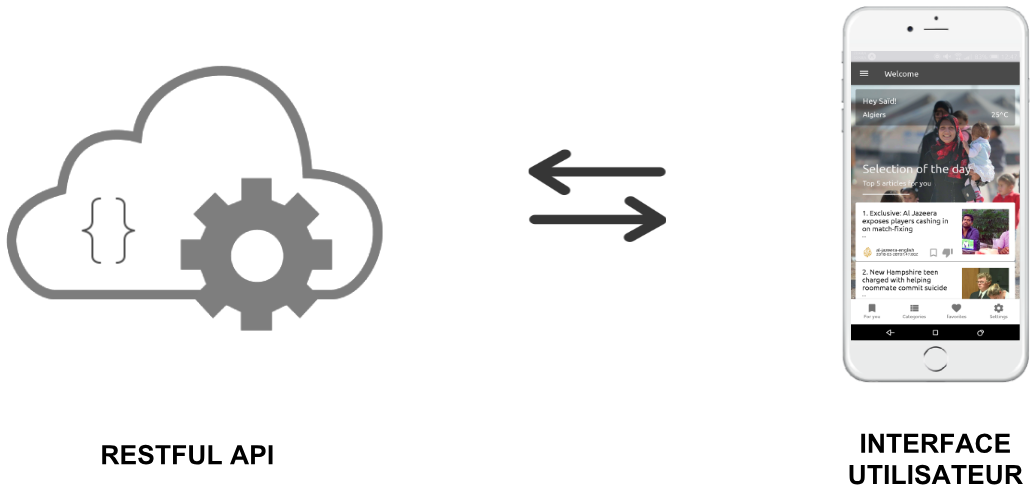
\includegraphics[height=132pt,width=270pt]{img/chapter4/frontbackend.png}
    \caption{API et application mobile - les deux composantes principales de \textquotedbl Feedny\textquotedbl. }
    \label{frontbackend}
\end{figure}

Nous allons présenter chaque composant apparu sur la \autoref{frontbackend} et ses étapes d'implémentations en détail dans ce qui suit.

\subsection{Développement Back-end}
La partie \textquotedbl métier\textquotedbl de l'application consiste en un service web sous l'architecture REST\footnote{Respresentational State Transfert : un style d'architecture définissant un ensemble de contraintes et de propriétés basées sur le protocole HTTP [Wikipédia]} API\footnote{Application Programming Interface : un ensemble normalisé de classes, de méthodes ou de fonctions qui sert de façade par laquelle un logiciel offre des services à d'autres logiciels [Wikipédia]} qui intègre tous les modules. L'API reçoit les requêtes des utilisateurs à travers l'interface, et retourne une réponse via le protocole HTTP. Le Back-end est développé entièrement en Python en utilisant le Framework Flask\autoref{flask}. L'API est hébergée, pendant la phase de développement, sur un serveur web. 

Elle est composée de deux modules :
\begin{itemize}
    \item Module d'extraction d'articles
    \item Module de gestion de la base de données
\end{itemize} 

\subsubsection{Extraction d'articles}
Le composant le plus important dans notre système est l'article de presse. Ce dernier se trouve un peu partout sur les revues de presse en ligne. À cet effet, nous avons implémenté une fonctionnalité qui permet d'extraire des articles de presse de différentes sources dans les deux langues. L'extraction d'articles de presse peut être personnalisée selon le besoin; on peut choisir des articles à partir des catégories, région, pays, etc.

Lors de l'extraction d'un article, nous récupérons toutes les informations relatives à ce dernier tels que le contenu de l'article, le titre, l'auteur, l'horaire de publication, etc.

Le module d'extraction d'articles de presse peut être invoqué juste en saisissant une requête dans le navigateur ou en visitant la page principale de notre application. La réponse est retournée sous le format JSON, comme dans l'exemple suivant qui monte une extraction par nom de source :

\begin{lstlisting}[style=api] 
http://feedny.io/api/articles/add/sources=al-jazeera-english
\end{lstlisting}

ou encore par catégorie :
\begin{lstlisting}[style=api] 
http://feedny.io/api/articles/add/categories=sport,health
\end{lstlisting}  

\subsubsection{Gestion de la base de données}
Le module de gestion de la base de données s'occupe de l'insertion, la suppression, la recherche et la mise à jour des articles et des profils utilisateurs. Chaque appel à l'API implique systématiquement une opération implicite sur la base de données. Elle est composée, comme cité dans la \autoref{concept-bdd}, de deux collections : Articles et Profils. 

       \begin{enumerate}[leftmargin=*]
    \item\textbf{Gestion de la collection d'Articles}\\
    Après extraction d'un article de presse, il sera stocké dans un document qui appartient à la collection Articles dans notre base de données NoSQL afin de faciliter la recherche et de remédier à la lenteur du débit internet. (la structure d'un document Article a été présentée dans \autoref{article-collection})
    
    La recherche peut se faire avec n'importe quel attribut d'un article de presse, et c'est l'un des plus grands avantages des bases de données NoSQL. Les articles peuvent aussi avoir une structure différente, et on peut stocker, également, des images et du son, s'il y en a. On peut également proposer des articles à un utilisateur, en utilisant son vecteur de probabilité de sélection et ses sources préférées : 
    
    \begin{lstlisting}[style=api] 
    http://feedny.io/api/profiles/onload/username=yankheloufi
    \end{lstlisting} 

\item\textbf{Gestion de la collection de Profils}\\
La structure des profils utilisateurs est très dynamique; elle est différente d'un utilisateur à un autre. Les utilisateurs peuvent avoir plusieurs préférences et sources favorites. La gestion des profils est également effectuée à partir de l'API. 
Un nouvel utilisateur est ajouté de la façon suivante :   
\begin{lstlisting}[style=api] 
http://feedny.io/api/profiles/add/profile=username::password::user@hey.com::sport,religion::bbc-news,echourouk
\end{lstlisting} 

Et le profil peut être également mis à jour de la manière qui suit : 
\begin{lstlisting}[style=api] 
http://feedny.io/api/profiles/update/profile=username::preferences+algeria
\end{lstlisting}            
\end{enumerate} 

\subsection{Développement Front-end}
Dans le monde du développement web et mobile, nous recherchons toujours des cycles de développement très courts, des délais de déploiement réduits avec une meilleure performance. Une technologie très récente (2016) se trouve au beau milieu de ces exigences, le développement d'application mobile hybride en utilisant des techniques et des langages de programmation très répandus parmi les développeurs web (comme JavaScript ou HTML5 et CSS) enveloppés dans un Framework leur permettant de fonctionner nativement sur n'importe quel appareil et système d'exploitation (Androïd ou IOS).

Il existe plusieurs Frameworks d'applications mobiles hybrides, mais React-native (\autoref{react-native-def}) développé par \emph{Facebook} et, jusqu'à l'écriture de ces lignes, reste le plus performant et le plus évolutif tout en restant stable. On peut citer quelques points forts de React-native : 
\begin{itemize}
    \item Open source et communauté ne cessent de s'agrandir,
    \item Facebook continue à investir dans sa croissance,
    \item Les composants sont réutilisables,
    \item Compatibilité avec les APIs, les SGBDs et les extensions tiers,
    \item Moins d'utilisation de la mémoire,
    \item ...
\end{itemize}
Tous ces arguments nous ont poussés à choisir React-native comme Framework pour développer notre application mobile. 

\subsection{Fonctionnalités disponibles}
Deux méthodes d'utilisation de notre application sont disponibles. Avec authentification ou sans authentification. La personnalisation des recommandations en dépendra.
\begin{enumerate}[leftmargin=*]
    \item\textbf{Avec authentification (personnalisé)}\\
    Si l'utilisateur s'authentifie, la version personnalisée de notre application lui sera accessible et pourra dès la première connexion choisir ses catégories et ses sources favorites afin de construire son profil utilisateur.
    
    À partir de là, les articles proposés sont choisis en fonction de ses préférences, et les recommandations seront de plus en plus raffinées avec l'utilisation de l'application.
    
    Les utilisateurs de \textquotedbl Feedny\textquotedbl auront comme fonctionnalités:  
    \begin{itemize}
        \item \textbf{Catégorisation automatique d'articles :}\\
        Les articles sont classifiés dans différentes catégories suivant le sujet traité.
        \item \textbf{Résumé automatique :}\\
        Au lieu de lire un article complet, l'utilisateur aura un résumé généré automatiquement à partir de l'article qui lui permettra de retrouver tous les faits importants décrits dans l'article.
        \item \textbf{Traduction automatique :}\\
        L'utilisateur aura la possibilité d'avoir une traduction de l'article en cours de lecture.
        \item \textbf{Favoriser un article, une revue ou une catégorie :}\\
        L'utilisateur pourra aussi marquer un article, une source ou une catégorie précise d'articles comme favorite.
        \item \textbf{Mentionner la satisfaction :}\\
        Il aura la possibilité d'ajouter une mention de préférence \textquotedbl J'aime\textquotedbl ou \textquotedbl Je n'aime pas\textquotedbl sur la recommandation.
        \item \textbf{Recherche d'articles :}\\
        L'utilisateur aura la possibilité de faire une recherche spécifique des articles, et ce en se basant soit sur une recherche basée mots clés, une recherche basée sur une catégorie ou une recherche selon la source de l'article. 
        \item \textbf{Consultations des articles recommandés :}\\
        L'interface offrira la possibilité de consulter tous les détails concernant l'article (auteur, date de publication, etc.) 
    \end{itemize}
    Dès la connexion de l'utilisateur, ce dernier peut s'identifier en utilisant un nom d'utilisateur et un mot de passe ; sinon, il utilisera les services non personnalisés du système qui sont présentés dans le point suivant.\\

\item\textbf{Sans authentification (non personnalisé)}\\
Dans le cas où l'utilisateur ne souhaite pas s'identifier, la version non personnalisée sera entièrement accessible et il pourra faire :
\begin{itemize}
    \item \textbf{Une recommandation basée similarité :}\\
    Dans le cas non personnalisé, la recommandation se basera uniquement sur l'article consulté et lu et les différents articles disponibles dans la base de données.    
    \item \textbf{Une consultation des articles suggérés :}\\
    L’utilisateur pourra en effet au moment même où il lit un article, avoir une suggestion d'autres articles jugés similaires par le système.
    \item Toutes les autres fonctionnalités de la version personnalisée qui n'utilisent pas le profil utilisateur sont également disponibles.
\end{itemize}
\end{enumerate}
\vspace*{0.7cm}
Nous allons voir maintenant, les différentes interfaces de notre application.

\subsubsection{Authentification}
L'utilisateur peut créer un compte afin de s'authentifier, il peut s'inscrire en utilisant son compte \emph{Google}, \emph{Facebook} ou \emph{Twitter}.
Les informations relatives à l'authentification sont sauvegardées dans la collection des profils, ils seront utilisés tant que la session est ouverte.  
\begin{figure}[H]
    \centering
    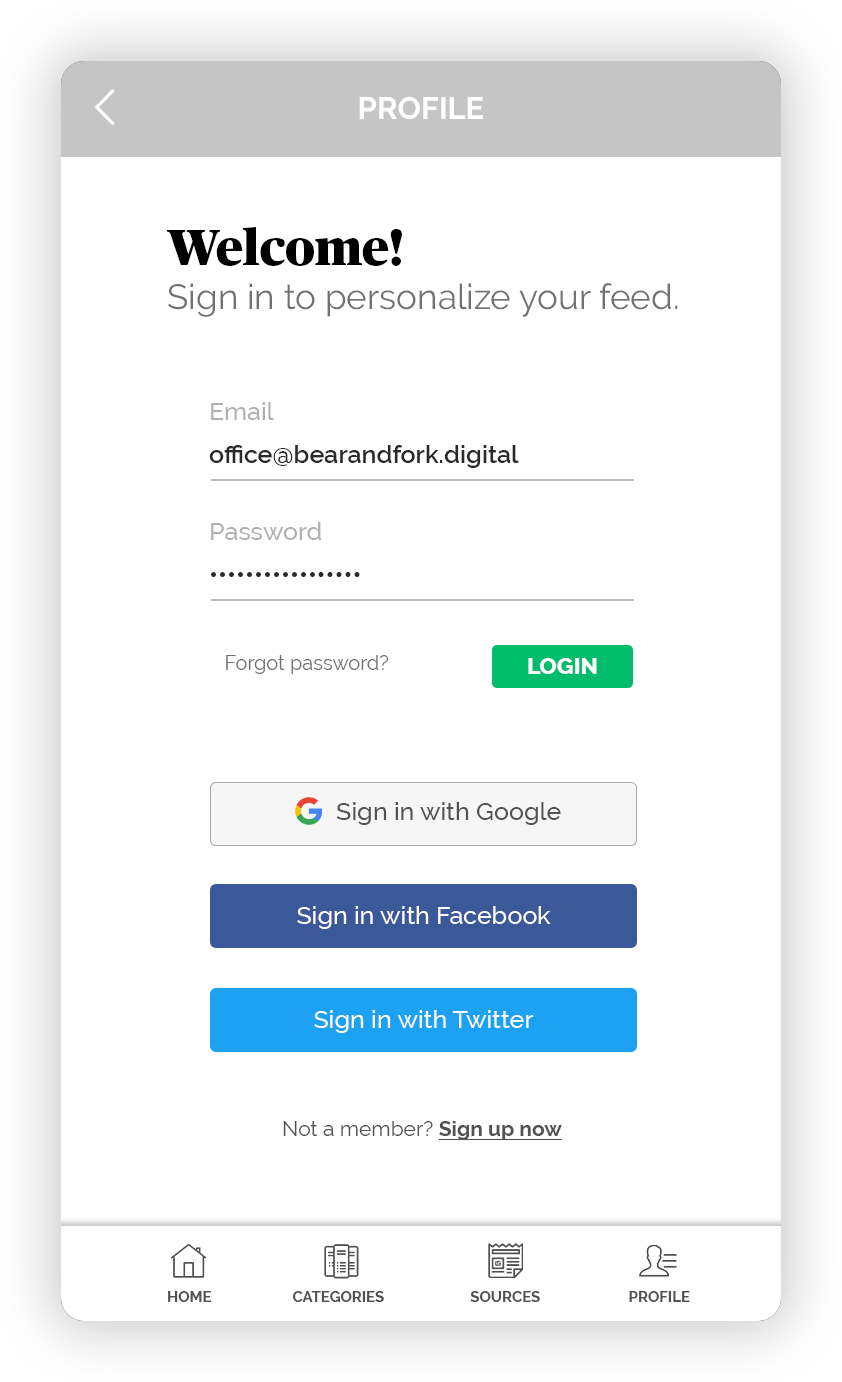
\includegraphics[width=140pt]{img/chapter4/feedny/en-sigin.png}
    \caption{Espace d'authentification de \textquotedbl Feedny\textquotedbl}
    \label{}
\end{figure}

\subsubsection{Accueil}
L'interface principale de \textquotedbl Feedny\textquotedbl (\autoref{home-display}). Les articles proposés sont affichés dans l'ordre de la pertinence, le premier article est le plus récent, mais aussi le plus adapté aux préférences de l'utilisateur.

\begin{figure}[H]
    \begin{minipage}{0.48\textwidth}
        \begin{figure}[H]
            \centering
            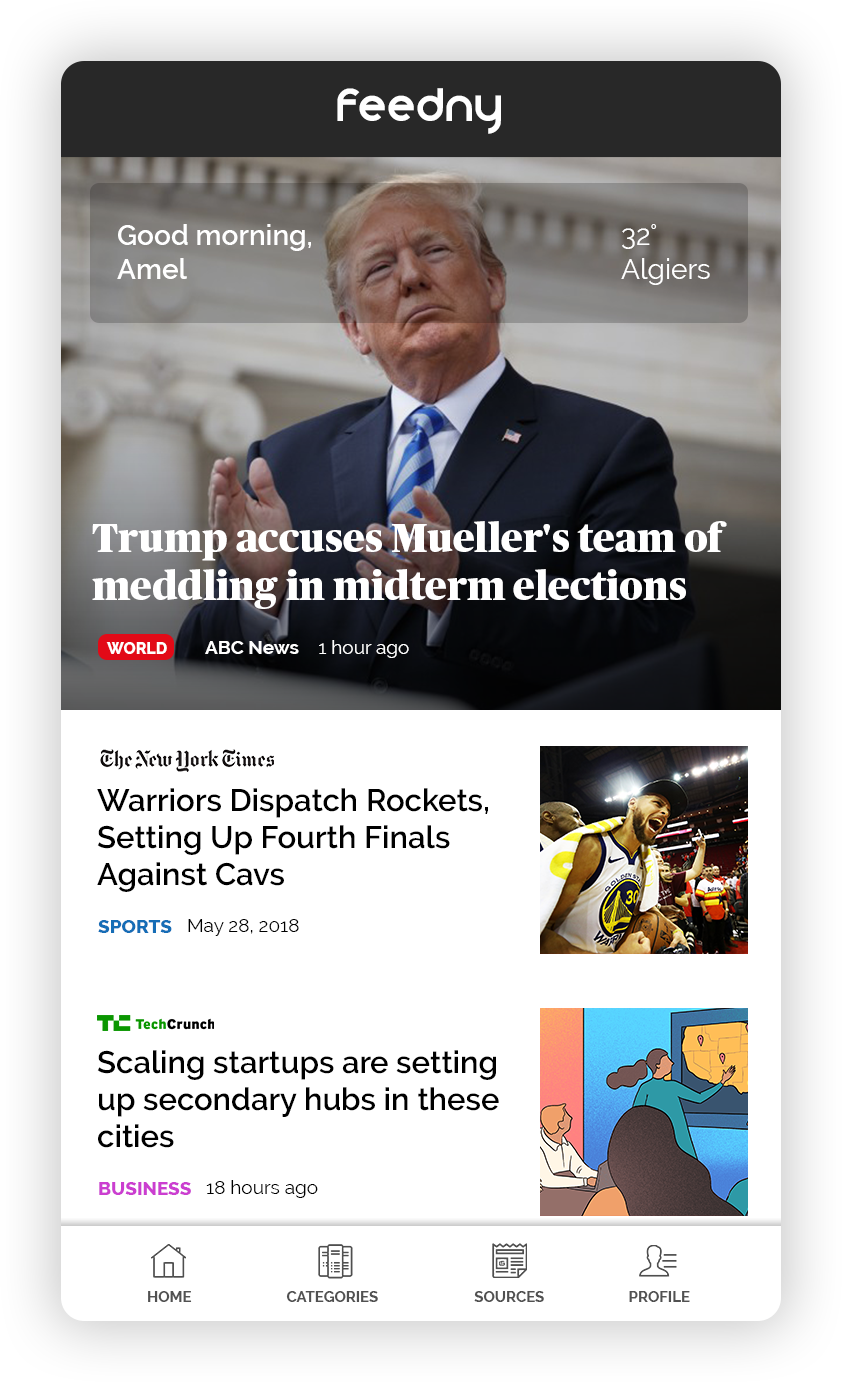
\includegraphics[width=140pt]{img/chapter4/feedny/en-home.png}
            \caption{Interface principale de \textquotedbl Feedny\textquotedbl en Anglais}
            \label{home-display}
        \end{figure}
    \end{minipage}\hfill
    \begin {minipage}{0.48\textwidth}
    \begin{figure}[H]
        \centering
        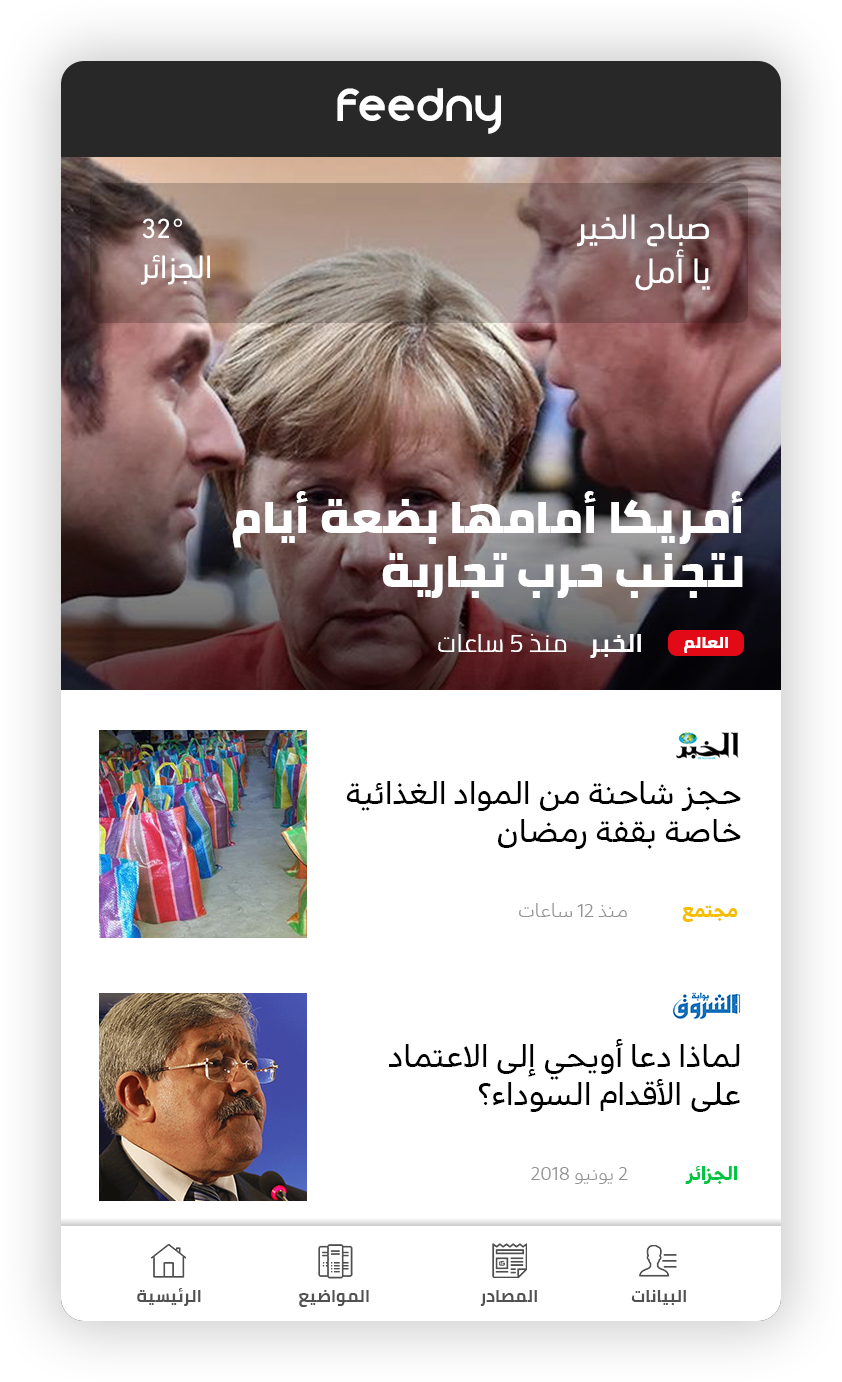
\includegraphics[width=140pt]{img/chapter4/feedny/ar-home.png}
        \caption{Interface principale de \textquotedbl Feedny\textquotedbl en Arabe}
        \label{}
    \end{figure}
\end{minipage}
\end{figure}


\subsubsection{Article}
Un article dans \textquotedbl Feedny\textquotedbl contient la catégorie inférée de l'article, l'image et la source sont affichés juste après, suivis du nom de l'auteur et la date de publication. Et enfin, le résumé généré et le contenu de l'article.   

\begin{figure}[H]
    \begin{minipage}{0.48\textwidth}
        \begin{figure}[H]
            \centering
            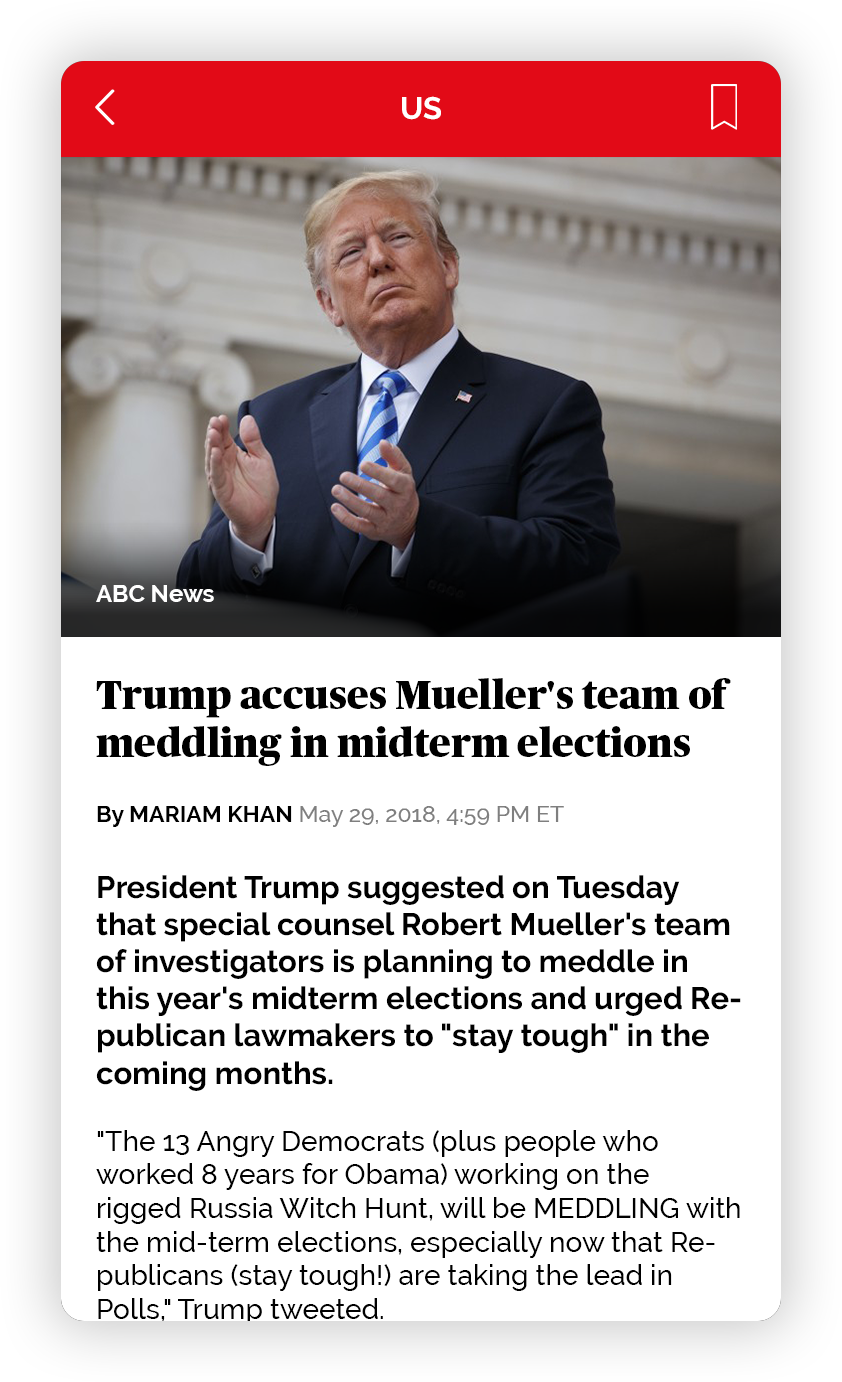
\includegraphics[width=140pt]{img/chapter4/feedny/en-article.png}
            \caption{Affichage des détails d'un article en langue Anglaise.}
        \end{figure}
    \end{minipage}\hfill
    \begin {minipage}{0.48\textwidth}
    \begin{figure}[H]
        \centering
        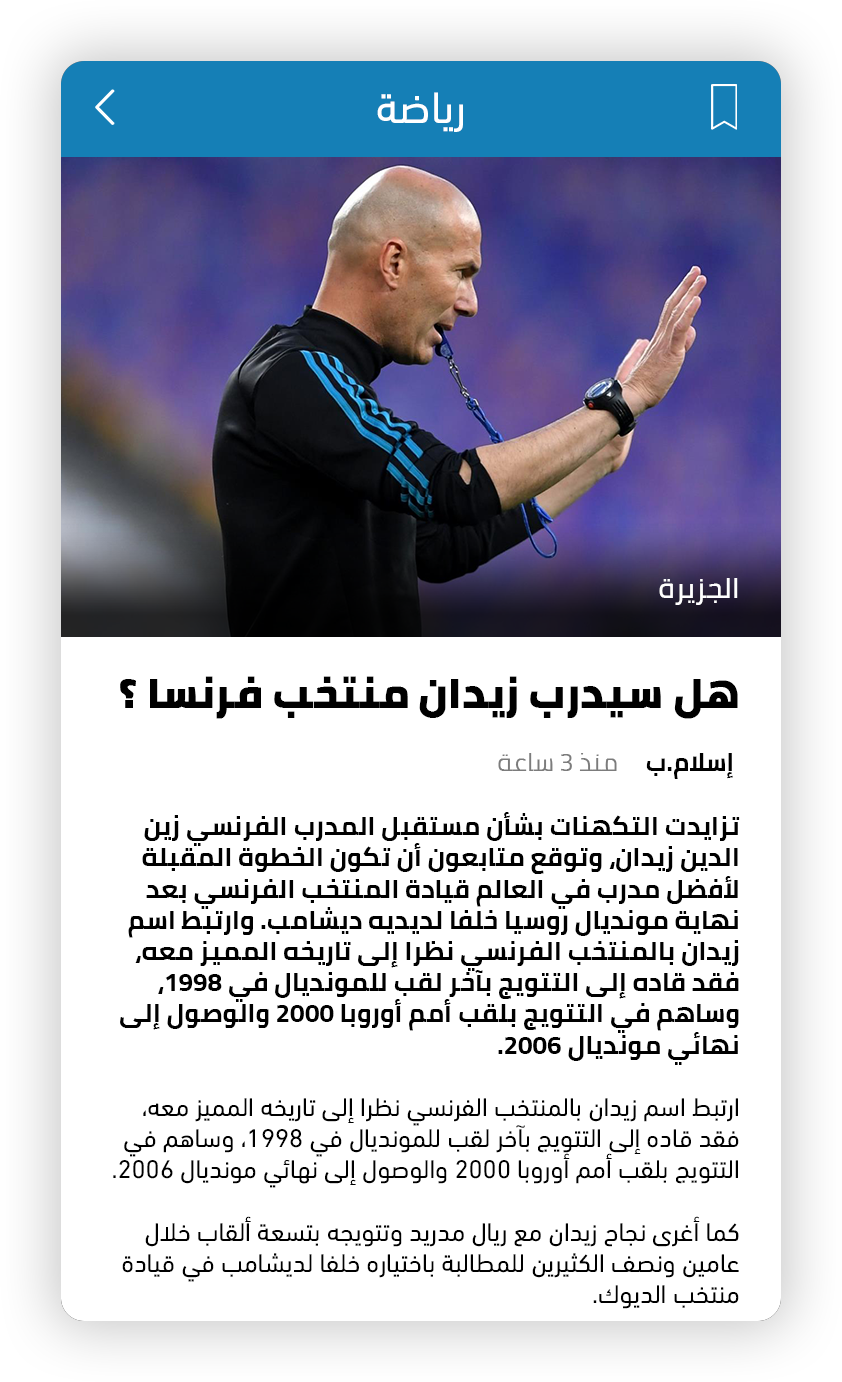
\includegraphics[width=140pt]{img/chapter4/feedny/ar-article.png}
        \caption{Affichage des détails d'un article en langue Arabe.}
    \end{figure}
\end{minipage}
\label{article-display}
\end{figure}

\subsubsection{Catégorie inférée et résumé généré}
La \autoref{categ-sum} présente le résumé généré d'un article et la catégorie inférée.
\begin{figure}[H]
    \centering
    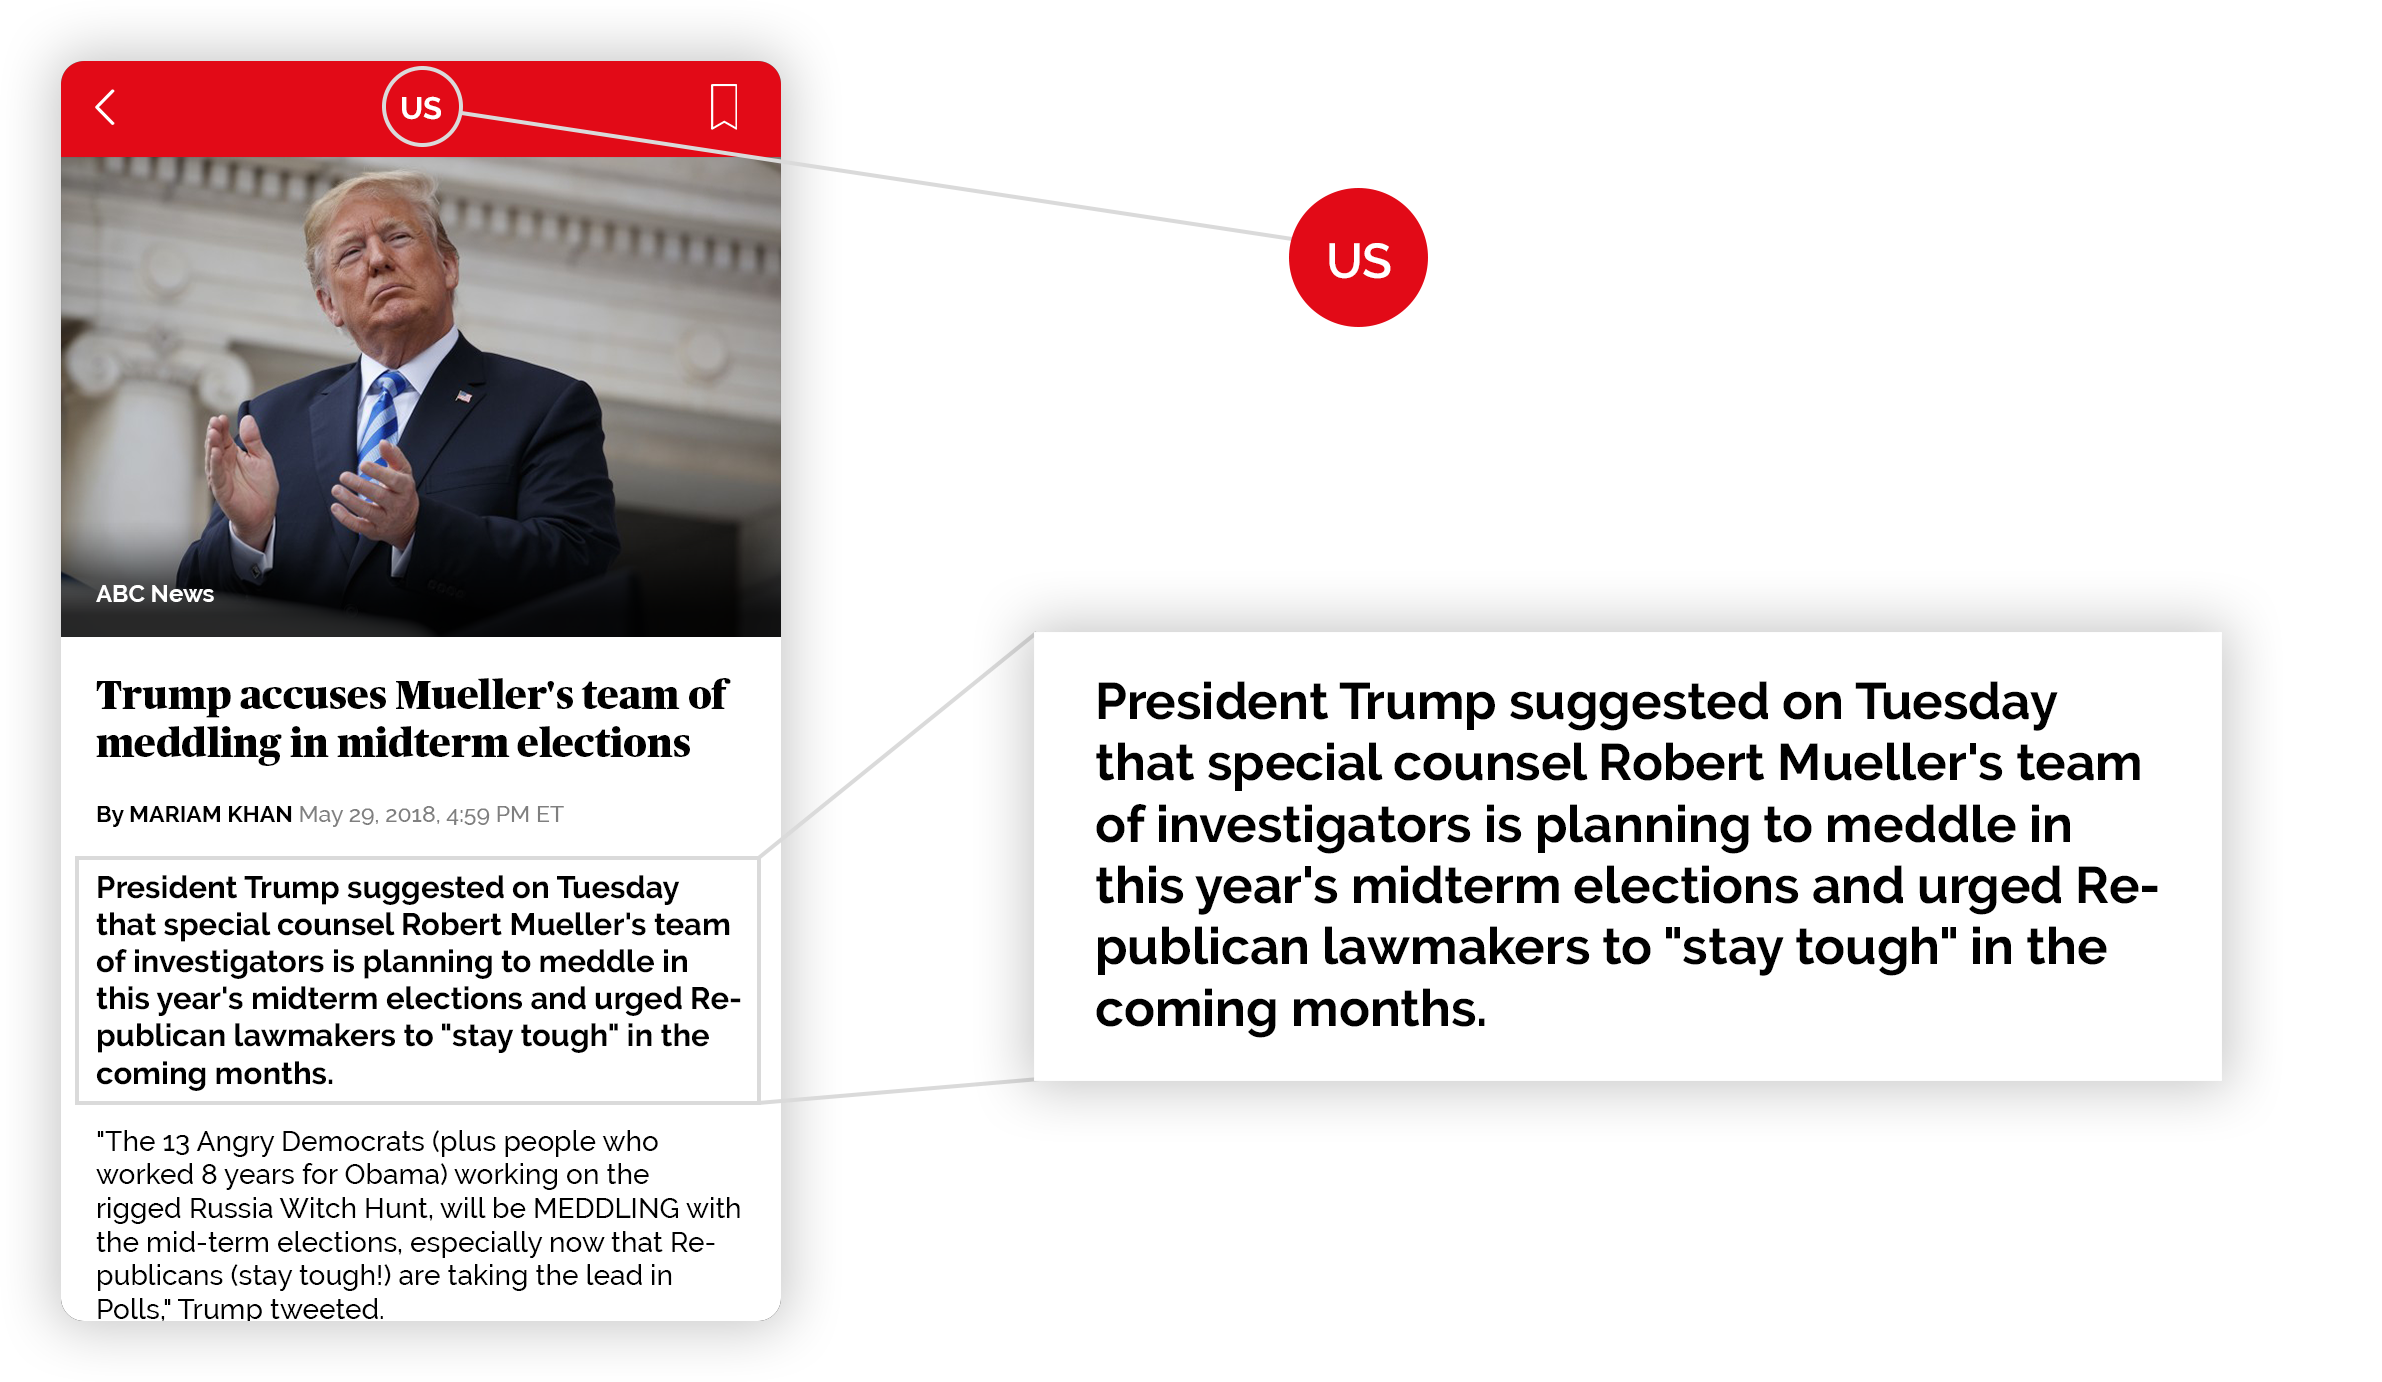
\includegraphics[width=410pt]{img/chapter4/feedny/en-summary.png}
    \caption{Gros plan sur la catégorie et le résumé généré par \textquotedbl Feedny\textquotedbl.}
    \label{categ-sum}
\end{figure}

\begin{figure}[H]
    \centering
    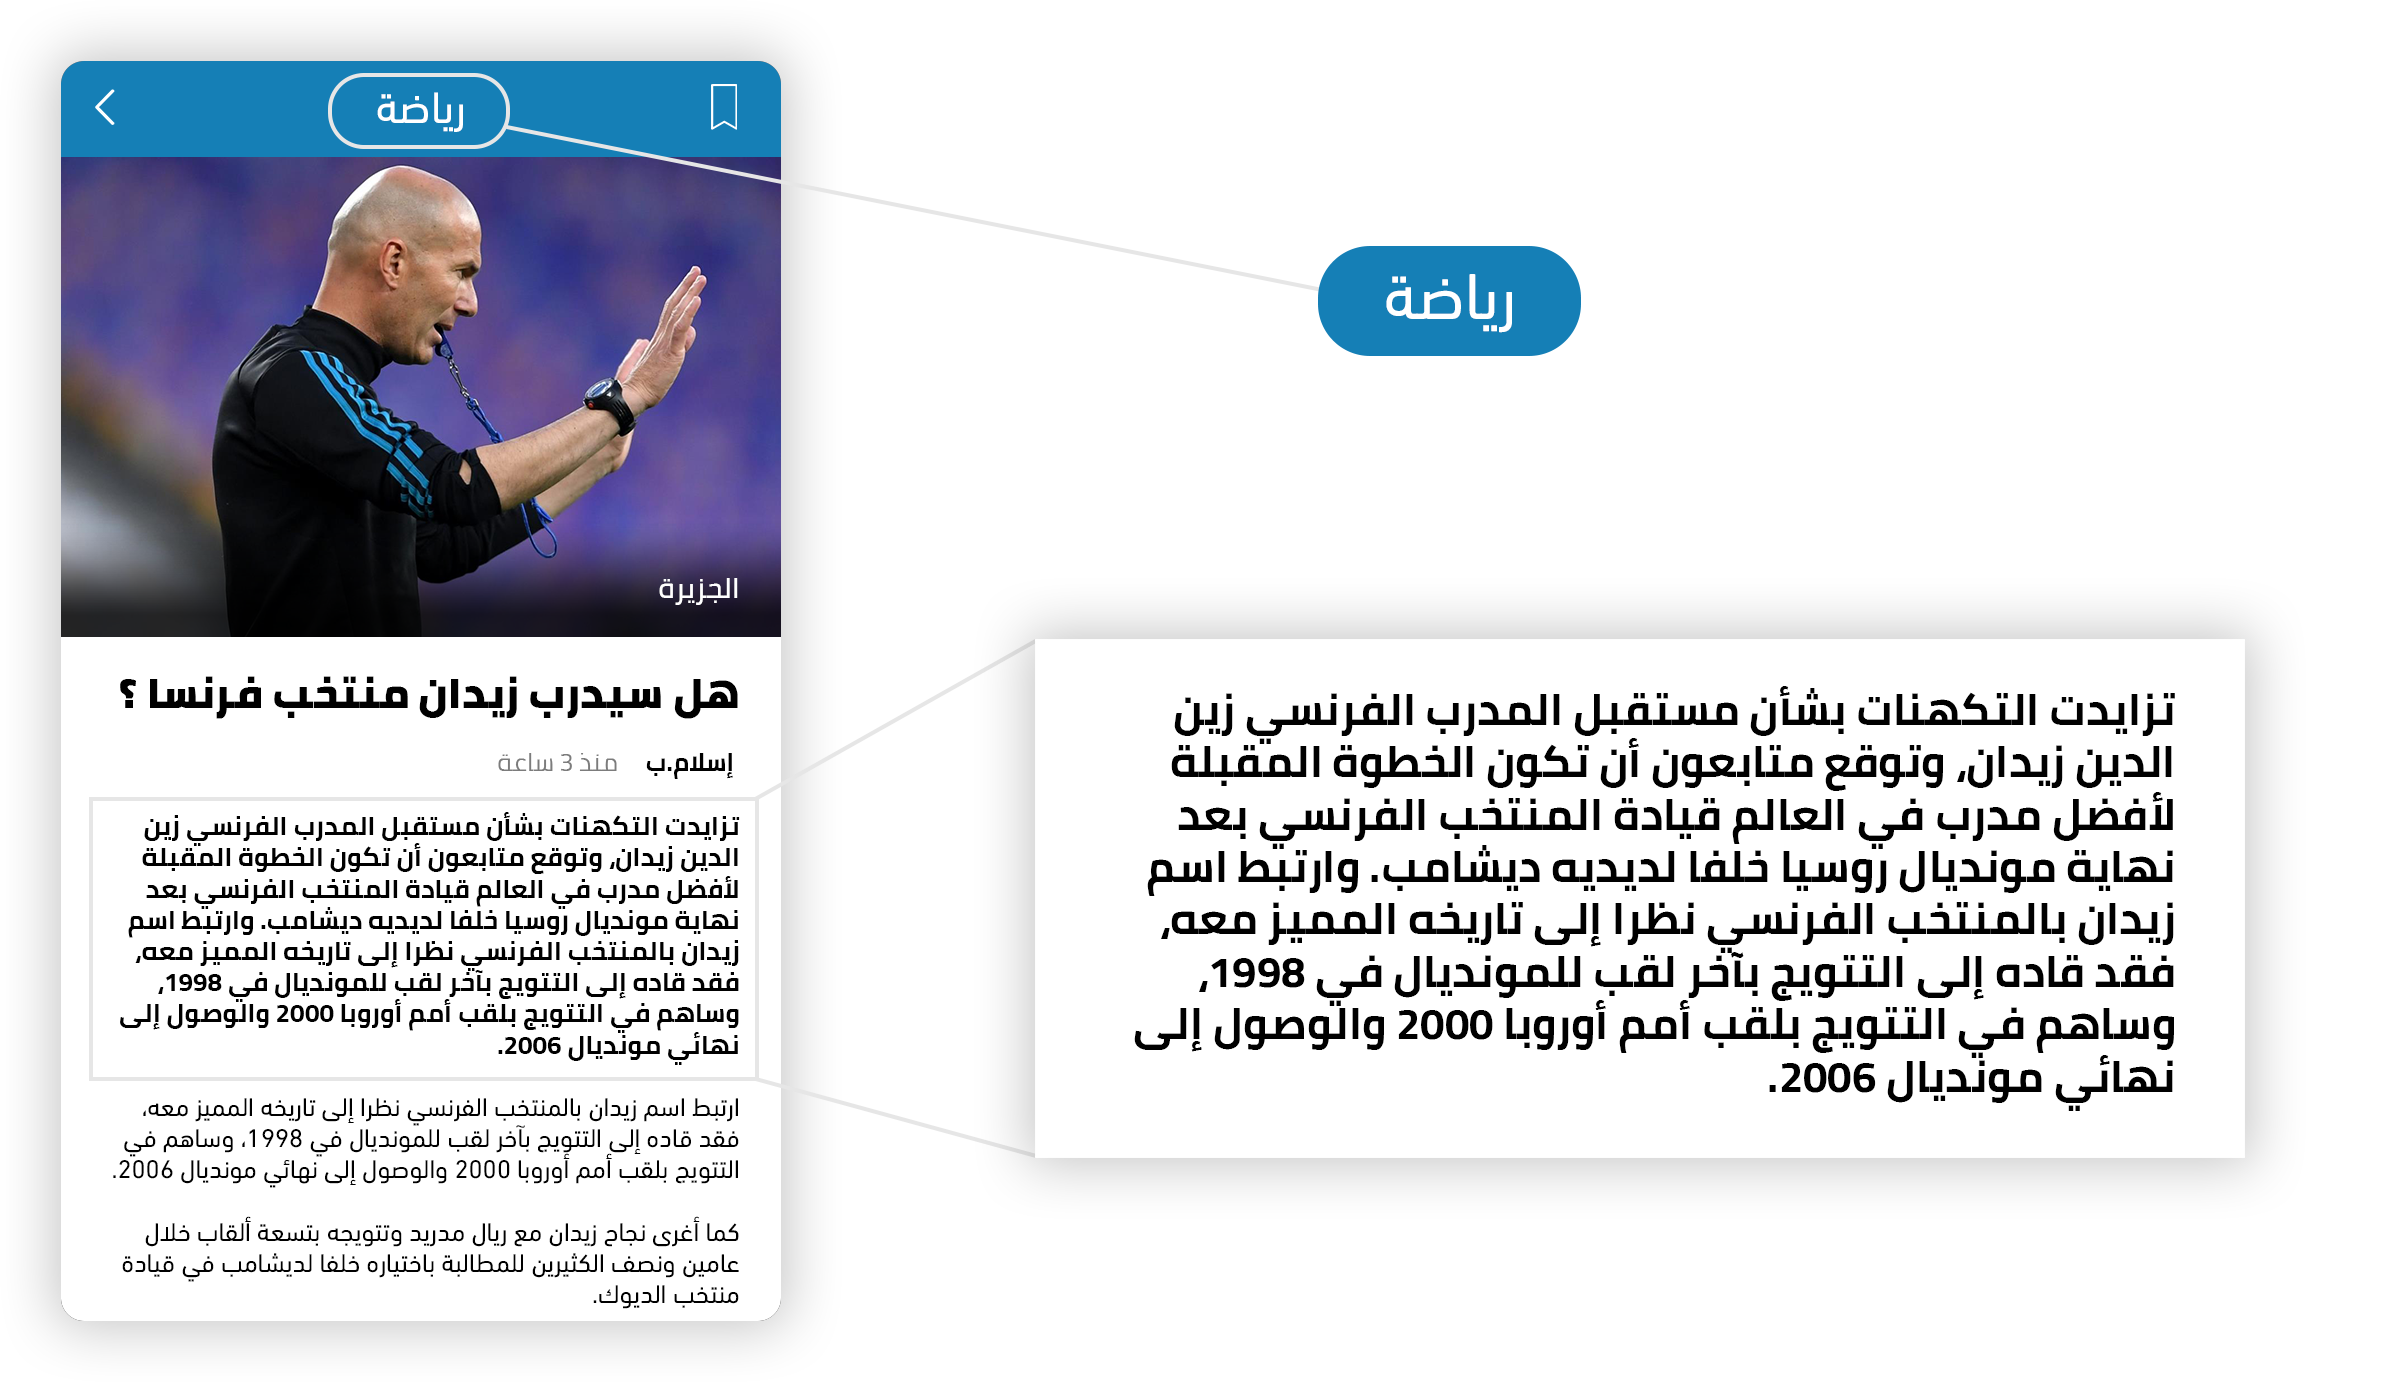
\includegraphics[width=410pt]{img/chapter4/feedny/ar-summary.png}
    \caption{Gros plan sur la catégorie et le résumé généré par \textquotedbl Feedny\textquotedbl.}
    \label{categ-sum}
\end{figure}

\subsubsection{Profil utilisateur}
L'interface présentée dans la \autoref{profile-display} contient les catégories et les sources préférées, mais aussi les articles que l'utilisateur a marqués comme favoris ou pour lire plus tard. L'utilisateur peut se déconnecter, ou se connecter s'il ne l'est pas déjà.
\begin{figure}[H]
    \centering
    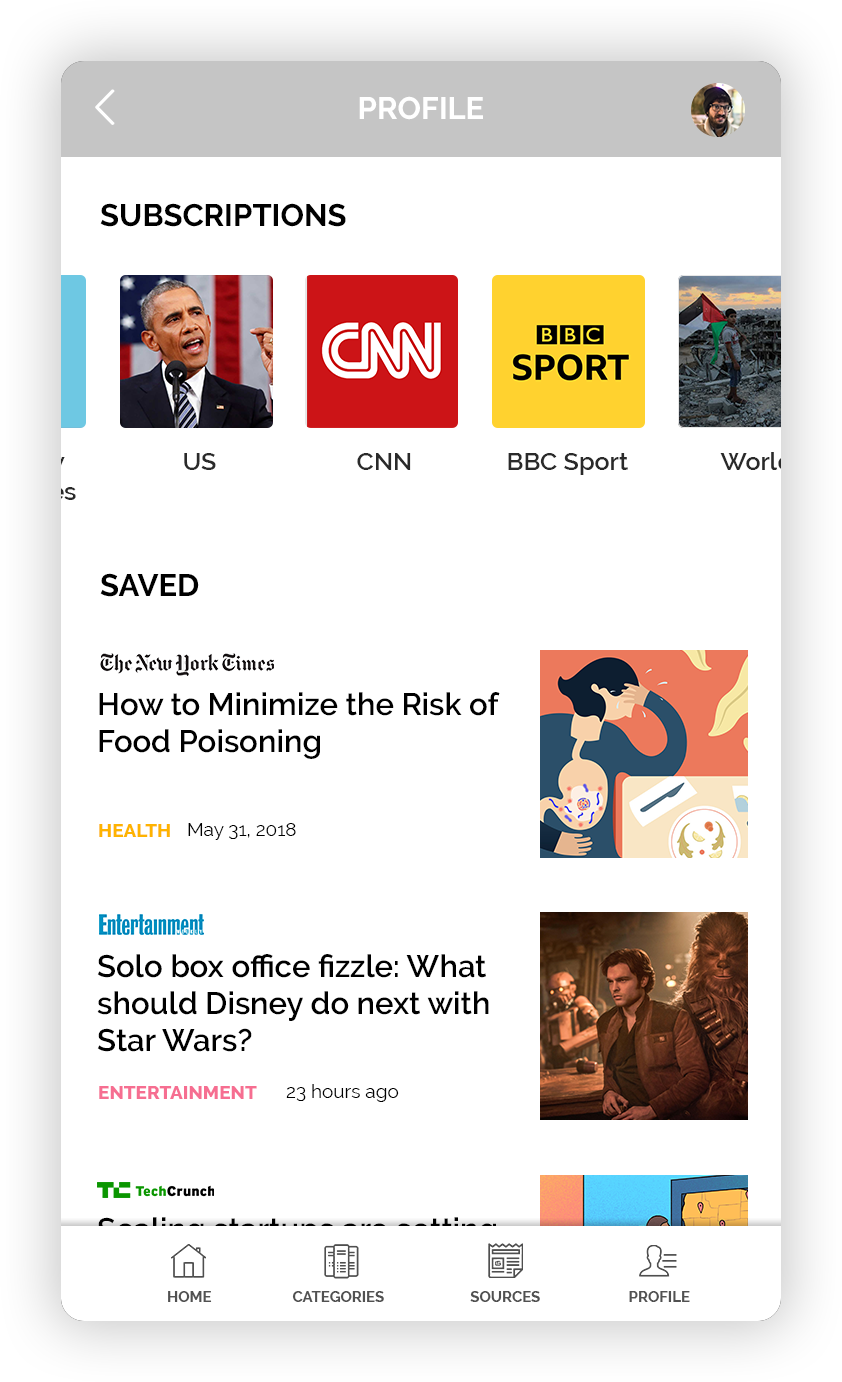
\includegraphics[width=140pt]{img/chapter4/feedny/en-profile.png}
    \caption{Détails sur le profil utilisateur}
    \label{profile-display}
\end{figure}

   \subsubsection{Catégories}
Toutes les catégories d'articles de presse de notre système sont regroupées dans l'interface présentée dans la \autoref{categ-display}, l'utilisateur peut favoriser des catégories ce qui va affecter les suggestions et les recommandations d'articles. 
\begin{figure}[H]
    \begin{minipage}{0.48\textwidth}
        \begin{figure}[H]
            \centering
            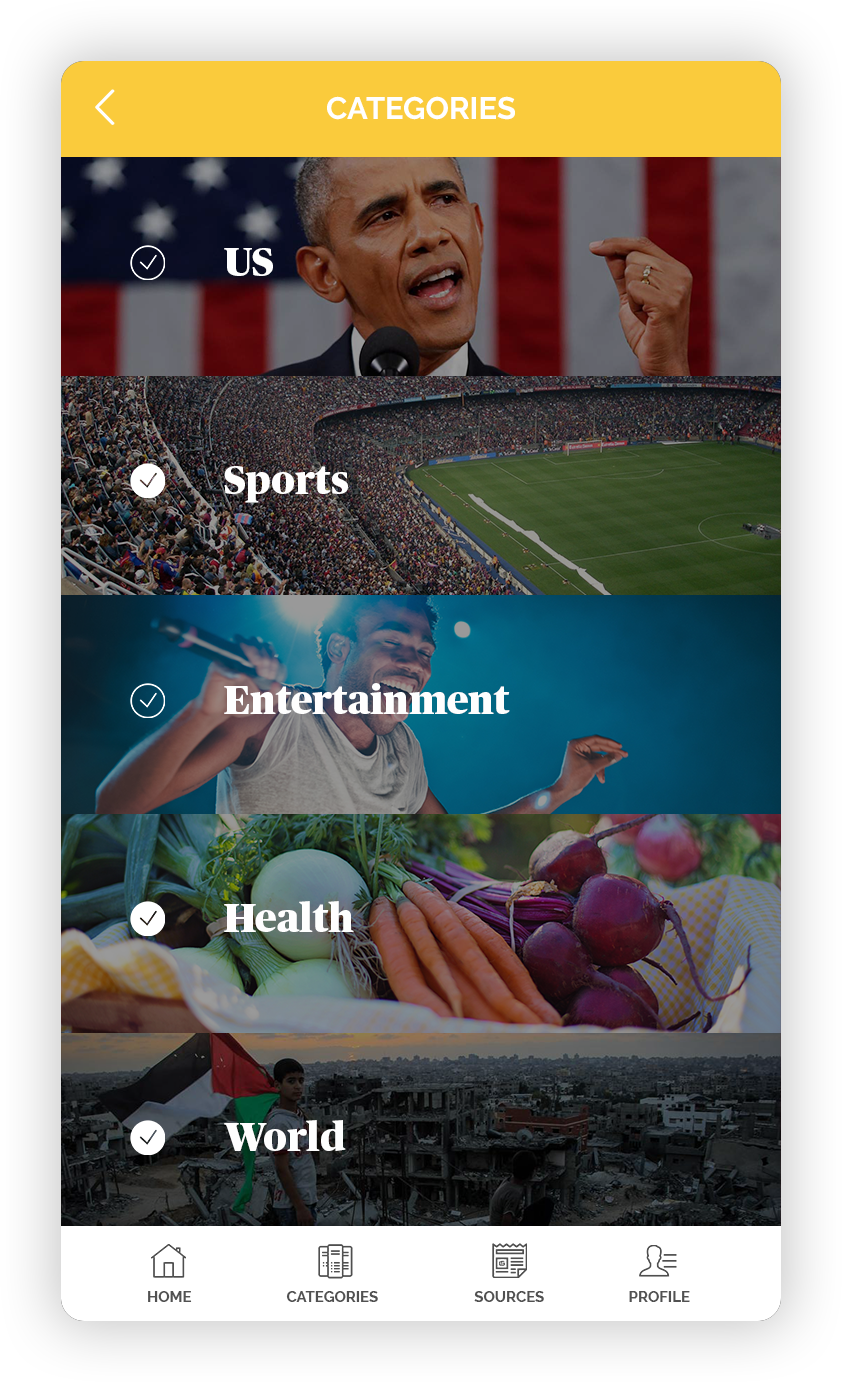
\includegraphics[width=140pt]{img/chapter4/feedny/en-categ.png}
            \caption{Catégories d'articles de presse de la langue Anglaise.}
        \end{figure}
    \end{minipage}\hfill
    \begin {minipage}{0.48\textwidth}
    \begin{figure}[H]
        \centering
        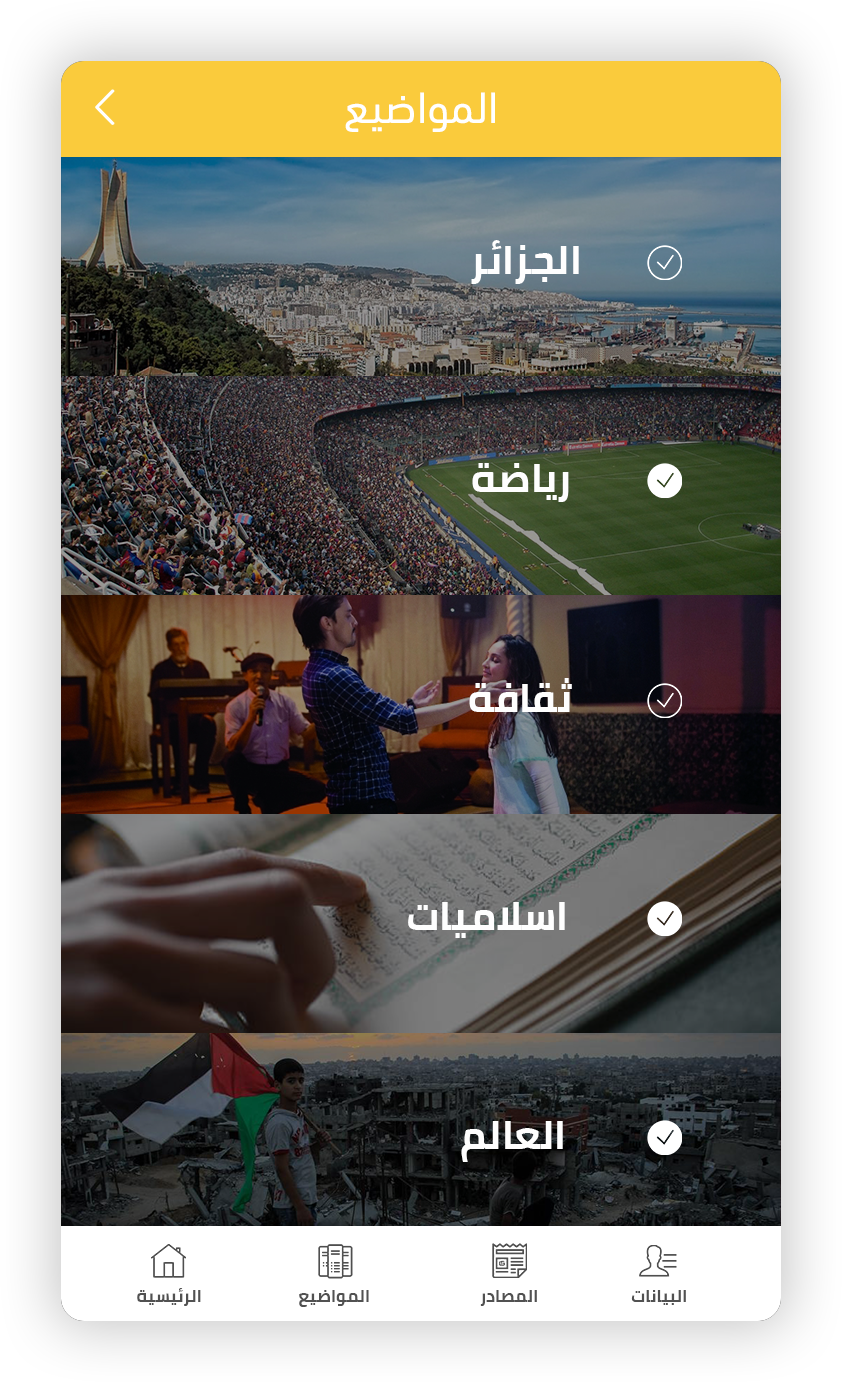
\includegraphics[width=140pt]{img/chapter4/feedny/ar-categ.png}
        \caption{Catégories d'articles de presse de la langue Arabe.}
    \end{figure}
\end{minipage}
\label{categ-display}
\end{figure}

\subsubsection{Articles par catégorie}
Cette figure (\autoref{article-categ}) présente l'interface utilisateur qui affiche tous les articles d'une seule catégorie. 
\begin{figure}[H]
    \centering
    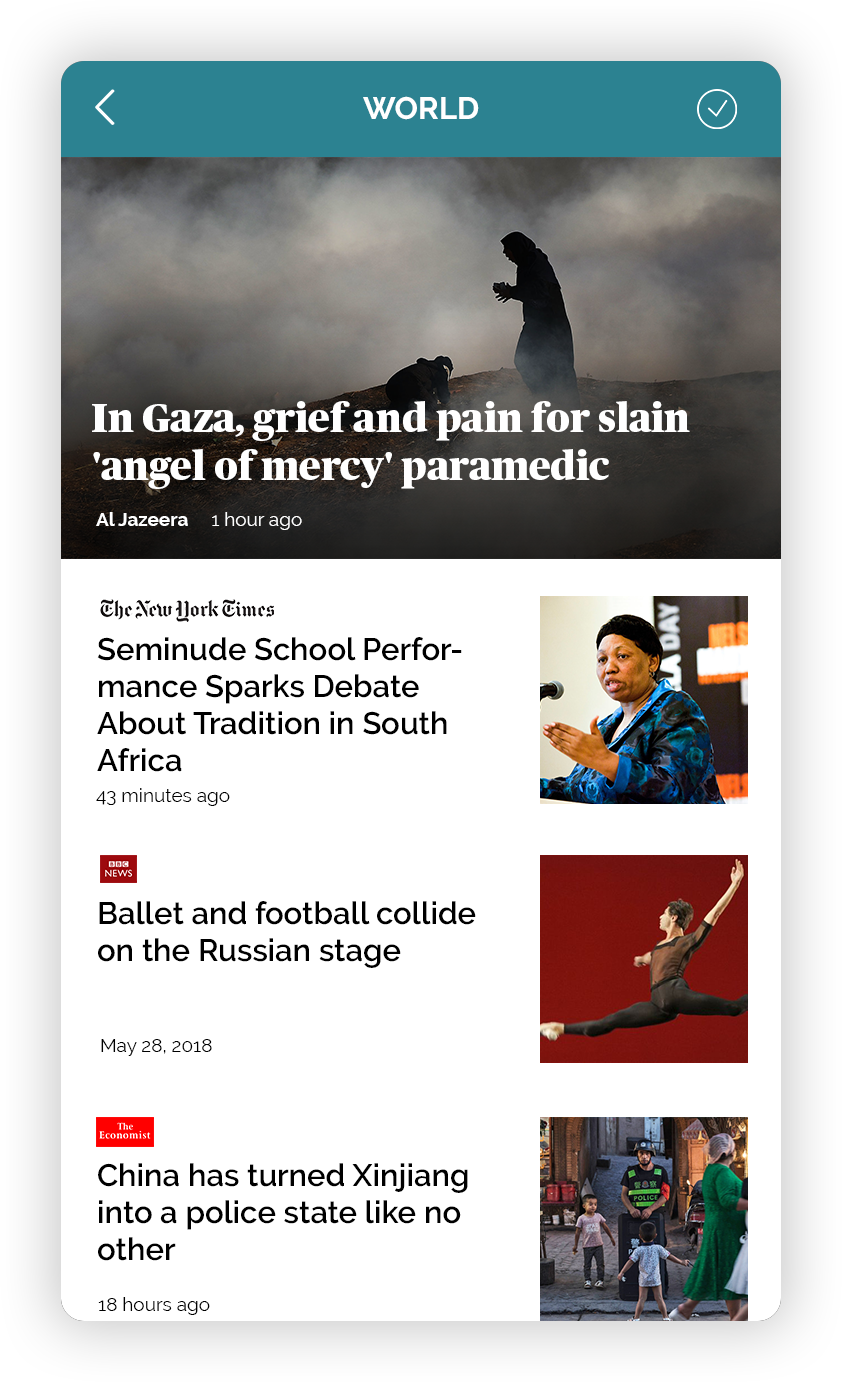
\includegraphics[width=140pt]{img/chapter4/feedny/en-categ-articles1.png}
    \caption{Tous les articles d'une catégorie.}
    \label{article-categ}
\end{figure}

La \autoref{article-categ2} contient une liste d'articles d'une catégorie donnée, trier par ordre de publication.
\begin{figure}[H]
    \centering
    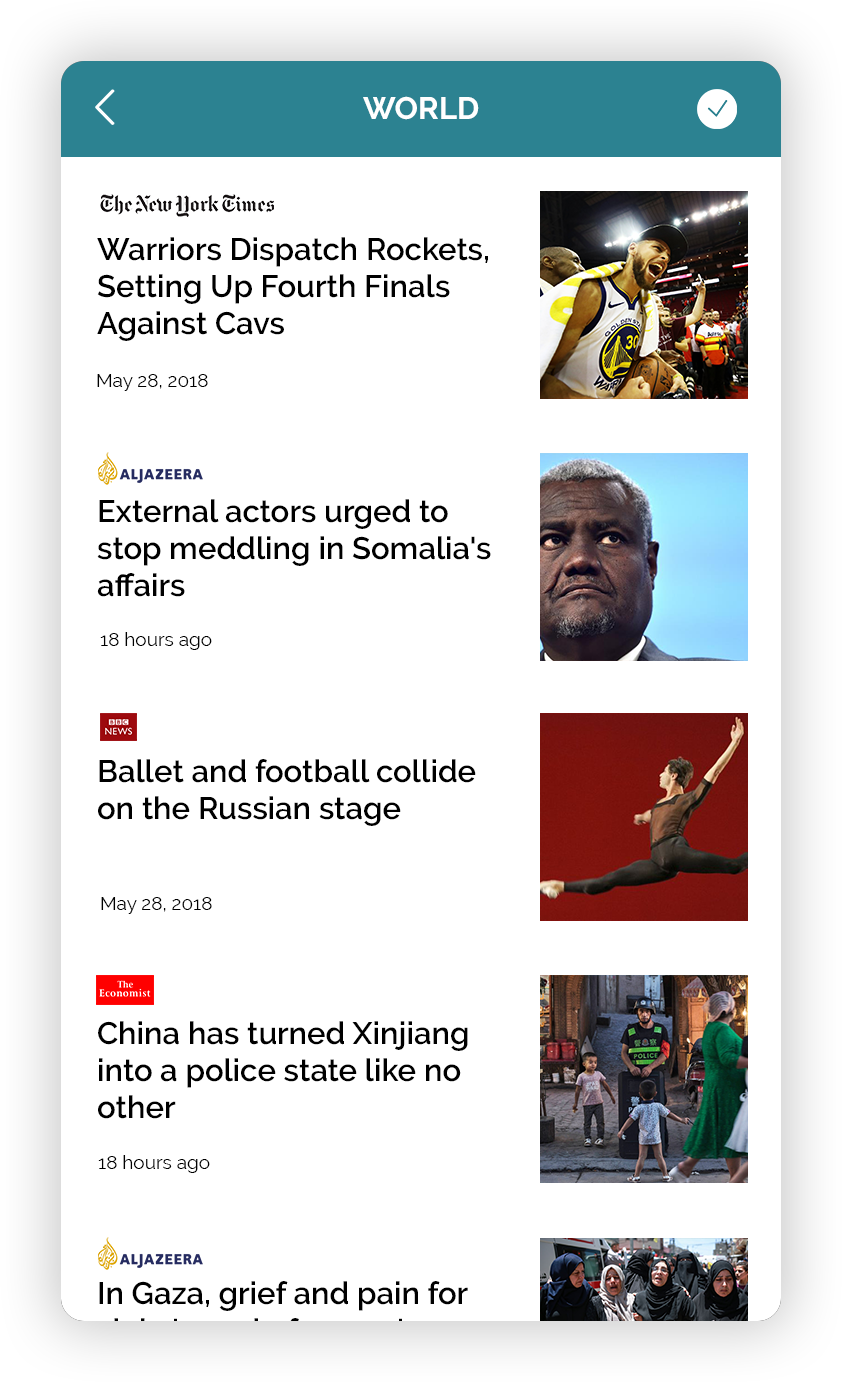
\includegraphics[width=140pt]{img/chapter4/feedny/en-categ-articles.png}
    \caption{Articles d'une catégorie trié par ordre de publication.}
    \label{article-categ2}
\end{figure}



 \subsubsection{Sources d'articles}
Les sources d'articles de presse (journaux, revue, etc.) sont présentées sur l'interface \emph{Sources}, l'utilisateur peut consulter les articles d'une source spécifique, mais aussi sélectionné des sources préférées.
\begin{figure}[H]
    \centering
    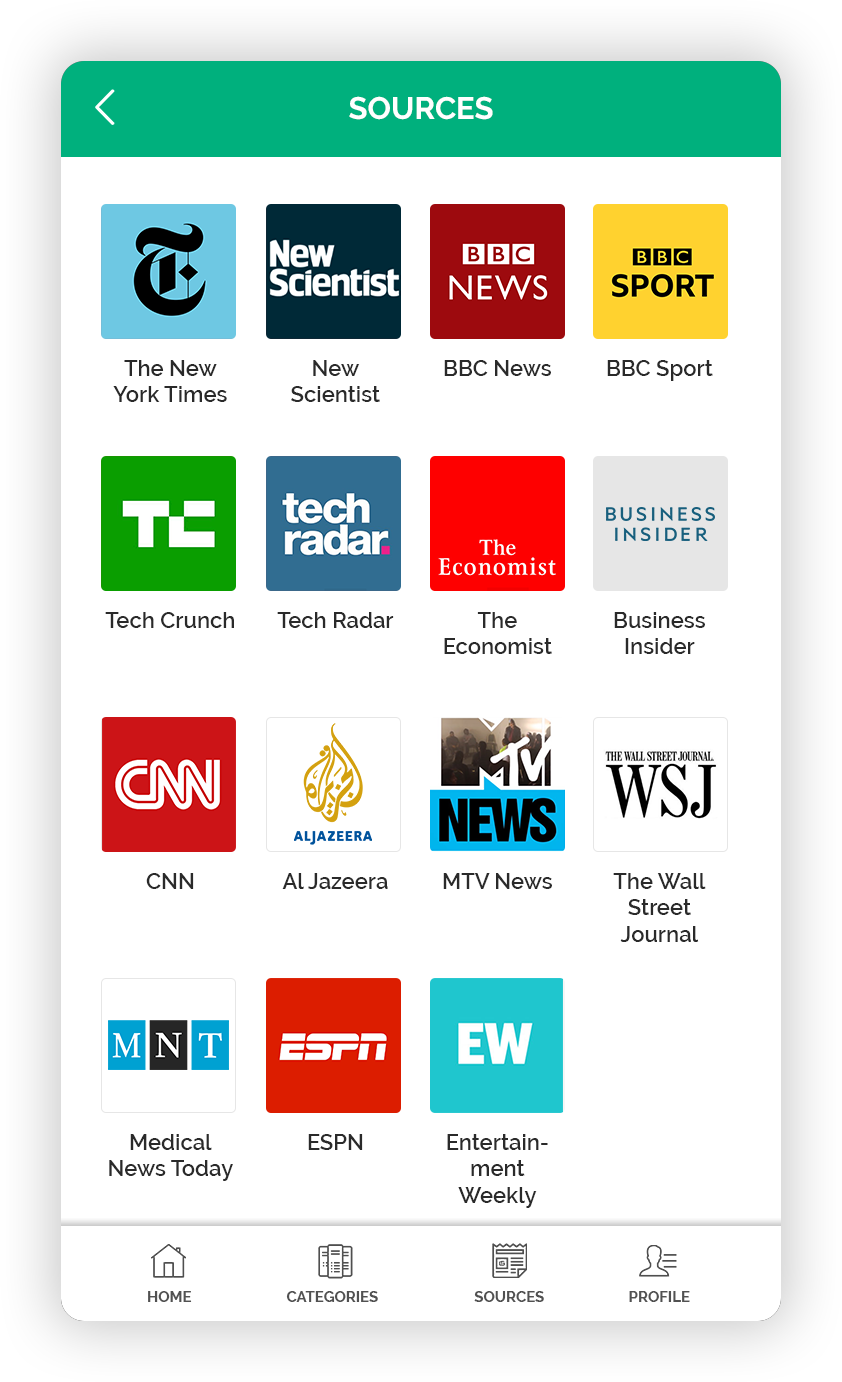
\includegraphics[width=140pt]{img/chapter4/feedny/en-sources.png}
    \caption{Sources d'articles de presse}
\end{figure}

Tous les articles qui appartient à un journal ou une revue de presse (Al Jazeera, BBC, etc.) peuvent être consulté en cliquant sur l'une des sources présentées dans la \autoref{sources-articles}.
\begin{figure}[H]
    \centering
    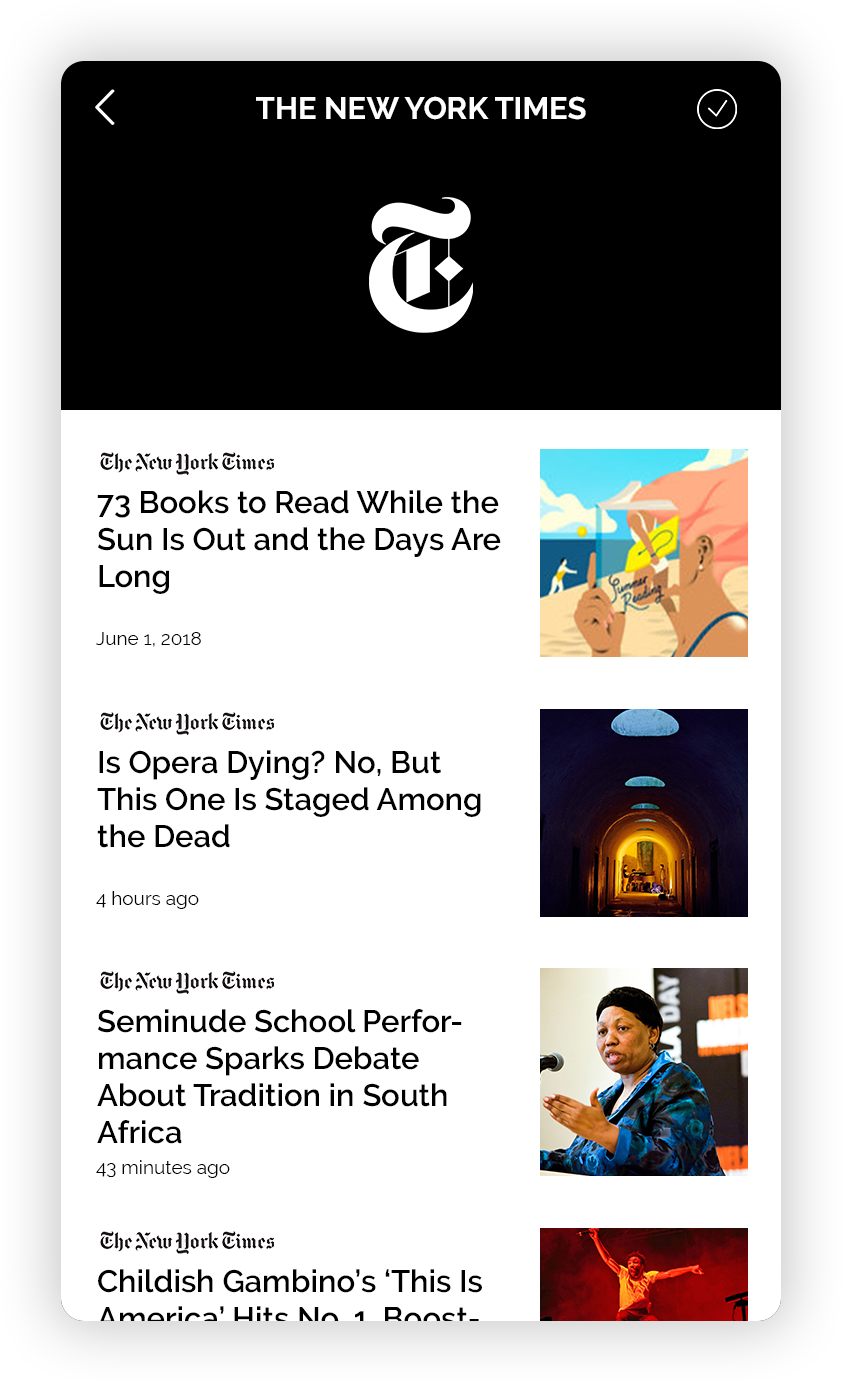
\includegraphics[width=140pt]{img/chapter4/feedny/en-articles-sources.png}
    \caption{Articles d'une source spécifique}
    \label{sources-articles}
\end{figure}

\section{Conclusion}
Dans ce chapitre, nous avons présenté les différents modules réalisés, les résultats obtenus et l'évaluation en utilisant les métriques adéquates. Nous avons présenté, également, l'environnement de travail, les librairies et les outils utilisés. Et enfin, nous avons parlé de l'intégration de chaque module dans \textquotedbl Feedny\textquotedbl ainsi que les fonctionnalités et les interfaces utilisateurs de notre application mobile.